\documentclass{mimosis}

% My packages
\usepackage{todonotes}
\usepackage{amsmath} % For definitions
\usepackage{threeparttable}
\usepackage{float}
\usepackage{metalogo}
\usepackage[T1]{fontenc}
\usepackage{subcaption}
%%%%%%%%%%%%%%%%%%%%%%%%%%%%%%%%%%%%%%%%%%%%%%%%%%%%%%%%%%%%%%%%%%%%%%%%
% Some of my favourite personal adjustments
%%%%%%%%%%%%%%%%%%%%%%%%%%%%%%%%%%%%%%%%%%%%%%%%%%%%%%%%%%%%%%%%%%%%%%%%
%
% These are the adjustments that I consider necessary for typesetting
% a nice thesis. However, they are *not* included in the template, as
% I do not want to force you to use them.

% This ensures that I am able to typeset bold font in table while still aligning the numbers
% correctly.
\usepackage{etoolbox}

\usepackage[binary-units=true]{siunitx}
\DeclareSIUnit\px{px}
% \newcommand{\todo}[1]{\textcolor{red}{(#1)}}
\newcommand{\bld}[1]{\textbf{#1}}

\sisetup{%
  detect-all           = true,
  detect-family        = true,
  detect-mode          = true,
  detect-shape         = true,
  detect-weight        = true,
  detect-inline-weight = math,
}


\usepackage[parfill]{parskip}

%%%%%%%%%%%%%%%%%%%%%%%%%%%%%%%%%%%%%%%%%%%%%%%%%%%%%%%%%%%%%%%%%%%%%%%%
% Hyperlinks & bookmarks
%%%%%%%%%%%%%%%%%%%%%%%%%%%%%%%%%%%%%%%%%%%%%%%%%%%%%%%%%%%%%%%%%%%%%%%%

\usepackage[%
  colorlinks = true,
  citecolor  = Green,
  linkcolor  = RoyalBlue,
  urlcolor   = RoyalBlue,
  unicode,
  ]{hyperref}

\usepackage{bookmark}

%%%%%%%%%%%%%%%%%%%%%%%%%%%%%%%%%%%%%%%%%%%%%%%%%%%%%%%%%%%%%%%%%%%%%%%%
% Bibliography
%%%%%%%%%%%%%%%%%%%%%%%%%%%%%%%%%%%%%%%%%%%%%%%%%%%%%%%%%%%%%%%%%%%%%%%%
%
% I like the bibliography to be extremely plain, showing only a numeric
% identifier and citing everything in simple brackets. The first names,
% if present, will be initialized. DOIs and URLs will be preserved.

\usepackage[%
  autocite     = plain,
  backend      = biber,
  doi          = true,
  url          = true,
  giveninits   = true,
  hyperref     = true,
  maxbibnames  = 99,
  maxcitenames = 99,
  sortcites    = true,
  style        = numeric,
  ]{biblatex}

%%%%%%%%%%%%%%%%%%%%%%%%%%%%%%%%%%%%%%%%%%%%%%%%%%%%%%%%%%%%%%%%%%%%%%%%
% Some adjustments to make the bibliography more clean
%%%%%%%%%%%%%%%%%%%%%%%%%%%%%%%%%%%%%%%%%%%%%%%%%%%%%%%%%%%%%%%%%%%%%%%%
%
% The subsequent commands do the following:
%  - Removing the month field from the bibliography
%  - Fixing the Oxford commma
%  - Suppress the "in" for journal articles
%  - Remove the parentheses of the year in an article
%  - Delimit volume and issue of an article by a colon ":" instead of
%    a dot ""
%  - Use commas to separate the location of publishers from their name
%  - Remove the abbreviation for technical reports
%  - Display the label of bibliographic entries without brackets in the
%    bibliography
%  - Ensure that DOIs are followed by a non-breakable space
%  - Use hair spaces between initials of authors
%  - Make the font size of citations smaller
%  - Fixing ordinal numbers (1st, 2nd, 3rd, and so) on by using
%    superscripts

% Remove the month field from the bibliography. It does not serve a good
% purpose, I guess. And often, it cannot be used because the journals
% have some crazy issue policies.
\AtEveryBibitem{\clearfield{month}}
\AtEveryCitekey{\clearfield{month}}

% Fixing the Oxford comma. Not sure whether this is the proper solution.
% More information is available under [1] and [2].
%
% [1] http://tex.stackexchange.com/questions/97712/biblatex-apa-style-is-missing-a-comma-in-the-references-why
% [2] http://tex.stackexchange.com/questions/44048/use-et-al-in-biblatex-custom-style
%
\AtBeginBibliography{%
  \renewcommand*{\finalnamedelim}{%
    \ifthenelse{\value{listcount} > 2}{%
      \addcomma
      \addspace
      \bibstring{and}%
    }{%
      \addspace
      \bibstring{and}%
    }
  }
}

% Suppress "in" for journal articles. This is unnecessary in my opinion
% because the journal title is typeset in italics anyway.
\renewbibmacro{in:}{%
  \ifentrytype{article}
  {%
  }%
  % else
  {%
    \printtext{\bibstring{in}\intitlepunct}%
  }%
}

% Remove the parentheses for the year in an article. This removes a lot
% of undesired parentheses in the bibliography, thereby improving the
% readability. Moreover, it makes the look of the bibliography more
% consistent.
\renewbibmacro*{issue+date}{%
  \setunit{\addcomma\space}
    \iffieldundef{issue}
      {\usebibmacro{date}}
      {\printfield{issue}%
       \setunit*{\addspace}%
       \usebibmacro{date}}%
  \newunit}

% Delimit the volume and the number of an article by a colon instead of
% by a dot, which I consider to be more readable.
\renewbibmacro*{volume+number+eid}{%
  \printfield{volume}%
  \setunit*{\addcolon}%
  \printfield{number}%
  \setunit{\addcomma\space}%
  \printfield{eid}%
}

% Do not use a colon for the publisher location. Instead, connect
% publisher, location, and date via commas.
\renewbibmacro*{publisher+location+date}{%
  \printlist{publisher}%
  \setunit*{\addcomma\space}%
  \printlist{location}%
  \setunit*{\addcomma\space}%
  \usebibmacro{date}%
  \newunit%
}

% Ditto for other entry types.
\renewbibmacro*{organization+location+date}{%
  \printlist{location}%
  \setunit*{\addcomma\space}%
  \printlist{organization}%
  \setunit*{\addcomma\space}%
  \usebibmacro{date}%
  \newunit%
}

% Display the label of a bibliographic entry in bare style, without any
% brackets. I like this more than the default.
%
% Note that this is *really* the proper and official way of doing this.
\DeclareFieldFormat{labelnumberwidth}{#1\adddot}

% Ensure that DOIs are followed by a non-breakable space.
\DeclareFieldFormat{doi}{%
  \mkbibacro{DOI}\addcolon\addnbspace
    \ifhyperref
      {\href{http://dx.doi.org/#1}{\nolinkurl{#1}}}
      %
      {\nolinkurl{#1}}
}

% Use proper hair spaces between initials as suggested by Bringhurst and
% others.
\renewcommand*\bibinitdelim {\addnbthinspace}
\renewcommand*\bibnamedelima{\addnbthinspace}
\renewcommand*\bibnamedelimb{\addnbthinspace}
\renewcommand*\bibnamedelimi{\addnbthinspace}

% Make the font size of citations smaller. Depending on your selected
% font, you might not need this.
\renewcommand*{\citesetup}{%
  \biburlsetup
  \small
}

\DeclareLanguageMapping{english}{english-mimosis}

\addbibresource{Thesis.bib}

%%%%%%%%%%%%%%%%%%%%%%%%%%%%%%%%%%%%%%%%%%%%%%%%%%%%%%%%%%%%%%%%%%%%%%%%
% Fonts
%%%%%%%%%%%%%%%%%%%%%%%%%%%%%%%%%%%%%%%%%%%%%%%%%%%%%%%%%%%%%%%%%%%%%%%%

\ifxetexorluatex
  \setmainfont{Minion Pro}
\else
  \usepackage[lf]{ebgaramond}
  \usepackage[oldstyle,scale=0.7]{sourcecodepro}
  \singlespacing
\fi

\renewcommand{\th}{\textsuperscript{\textup{th}}\xspace}

\newacronym {ANN}{ANN}{Artificial neural network}
\newacronym {CNN}{CNN}{Convolutional neural network}

% \newglossaryentry{LaTeX}{%
%   name        = {\LaTeX},
%   description = {A document preparation system},
%   sort        = {LaTeX},
% }

% \newglossaryentry{Real numbers}{%
%   name        = {$\real$},
%   description = {The set of real numbers},
%   sort        = {Real numbers},
% }

\makeindex
\makeglossaries




%%%%%%%%%%%%%%%%%%%%%%%%%%%%%%%%%%%%%%%%%%%%%%%%%%%%%%%%%%%%%%%%%%%%%%%%
% Incipit
%%%%%%%%%%%%%%%%%%%%%%%%%%%%%%%%%%%%%%%%%%%%%%%%%%%%%%%%%%%%%%%%%%%%%%%%

\title{Object Detection in Manufacturing Industry}
\subtitle{\textsc{Master's thesis}}
\author{Hai Duong Tran}

\begin{document}

\frontmatter
%   \begin{titlepage}

  \vspace*{1.5cm}
  \makeatletter

  \begin{center}
    \begin{LARGE}
        \textsc{Masaryk University}
    \end{LARGE}\\
    \begin{Large}
        \textsc{Faculty of Informatics}
    \end{Large}\\[1cm]
    
\includegraphics[width=4cm, height=4cm] {fi_logo.pdf}\\[2cm]
    \begin{Huge}
      \@title
    \end{Huge}\\[1.25cm]
    %
    \begin{Large}
      \@subtitle
    \end{Large}\\[1.5cm]
    \begin{LARGE}
    %
    \@author
    \end{LARGE}
    \vfill
    {\hfill\large Brno 2020}
  \end{center}
  \makeatother
\end{titlepage}

\newpage
\null
\thispagestyle{empty}
\newpage

%   \chapter*{Declaration}

\noindent
Hereby I declare, that this paper is my original authorial work, which I
have worked out by my own. All sources, references and literature used or
excerpted during elaboration of this work are properly cited and listed in
complete reference to the due source.
\vfill
\textbf{Advisor:} doc. RNDr. Pavel Matula, Ph.D.
%   \chapter*{Acknowledgements}
\noindent
Lorem ipsum dolor sit amet, consectetuer adipiscing elit. Temporibus autem quibusdam et aut officiis debitis aut rerum necessitatibus saepe eveniet ut et voluptates repudiandae sint et molestiae non recusandae. Proin in tellus sit amet nibh dignissim sagittis. Aliquam id dolor. Fusce dui leo, imperdiet in, aliquam sit amet, feugiat eu, orci. Sed vel lectus. Donec odio tempus molestie, porttitor ut, iaculis quis, sem. Nullam faucibus mi quis velit. Quisque porta. Integer pellentesque quam vel velit. Cum sociis natoque penatibus et magnis dis parturient montes, nascetur ridiculus mus.
%   \chapter*{Abstract}
\noindent
This work is concerned with object detection in images based on state-of-the-art
deep neural networks. The thesis is a result of a collaboration with
company SANEZOO EUROPE that provided image datasets. The work introduces
selected object detection models that were further evaluated according to
appropriate metrics on provided datasets. For future evaluations of the models
on an arbitrary datasets, we implemented a simple benchmarking tool that
can be controlled via web user interface.

\section*{Keywords}
\noindent
SANEZOO EUROPE, image processing, visual recognition, object detection, deep
learning, machine learning, neural networks, benchmarking

\tableofcontents

\mainmatter

\let\cleardoublepage\clearpage
%%%%%%%%%%%%%%%%%%%%%%%%%%%%%%%%%%%%%%%%%%%%%%%%%%%%%%%%%%%%%%%%%%%%%%%%
\chapter{Introduction}
%%%%%%%%%%%%%%%%%%%%%%%%%%%%%%%%%%%%%%%%%%%%%%%%%%%%%%%%%%%%%%%%%%%%%%%%

In the era of Industry 4.0, companies exploit modern technology to optimize traditional manufacturing and industrial processes. As human labor is expensive, companies search for new ways to minimize human assistance. Eyesight is one of the senses that could not be replaced easily for a long time. However, with recent advances in the field of computer vision, some human tasks can be done by robots that consist of camera systems that allow robots to perceive their surroundings. 

In 2015 scientists from Microsoft Research team proposed a deep learning model that surpassed human-level accuracy on a visual recognition task on the ImageNet 2012 classification dataset \cite{surp2015}. Since then, even better models were proposed \cite{resnet, efficientnet}. These high-performing image recognition models became the backbone of state-of-the-art object detection models, which are the key component of machine perception.

There are many areas where machine perception can be useful in industry. For instance, the models can be trained to detect faulty products soon enough to take corrective actions to ensure the products' quality. It is also a vital part of robotic arms that can carry out non-trivial tasks such as picking, sorting, and packing items. Another example of use can be observed in autonomous delivery navigation robots that can pick up trays of objects and move them around in a large warehouse~\cite{bmw}. 
%%%%%%%%%%%%%%%%%%%%%%%%%%%%%%%%%%%%%%%%%%%%%%%%%%%%%%%%%%%%%%%%%%%%%%%%
\chapter{Background}
%%%%%%%%%%%%%%%%%%%%%%%%%%%%%%%%%%%%%%%%%%%%%%%%%%%%%%%%%%%%%%%%%%%%%%%%
In this chapter, we first outline the aims and approaches of solving the object detection task. We then describe the fundamentals of deep learning for a better understanding of our chosen object detection models.

\section{Object Detection}

Object detection aims to locate objects in a given image and assign them to their \bld{class} (also called category or label). For illustration see Figure \ref{fig:od}. Generally, the task can be broken down into three steps: \bld{informative region selection}, \bld{feature extraction}, and \bld{classification}. In the first step, the method has to determine regions to which we apply the feature extraction. The feature extractor outputs a semantic numerical representation for each selected region is then used to predict the target's class. Note that, these steps are not fixed and the pipeline can vary.

\begin{figure}[h]
    \centering
    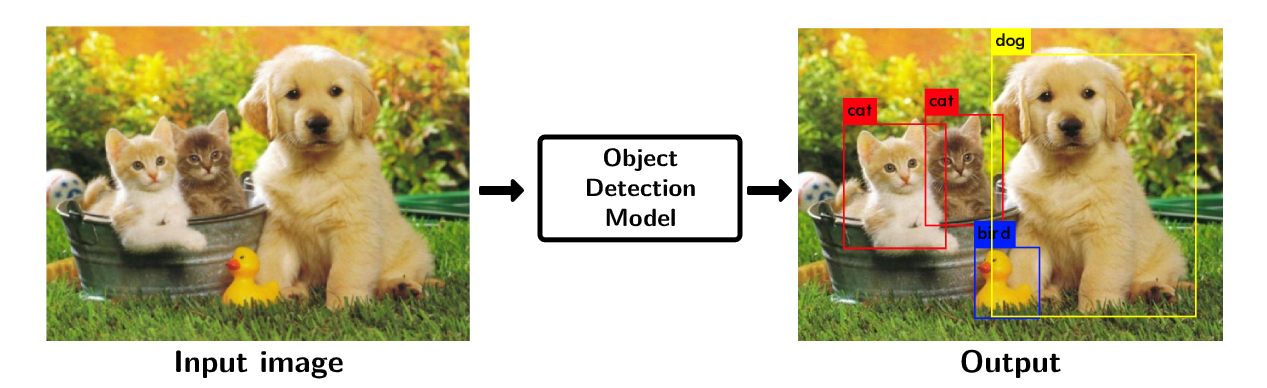
\includegraphics[width=0.9\linewidth]{Sources/Figures/objectdetection.png}
    \caption{A high-level illustration of an object detection pipeline. Adapted from \cite{objectdetectionfigure}.}
    \label{fig:od}
\end{figure}

Traditionally, engineers had to hand-craft feature extractors using algorithms such as SIFT \cite{sift}, SURF \cite{surf}, or HOG \cite{hog}. These methods are combined with well-established classification algorithms such as Support Vector Machines (SVM) \cite{svm}. Since this approach needs manual designing, it can be very demanding.

Deep learning methods introduced an end-to-end learning approach, which means that the model only takes a given set of annotated images to learn to detect key features, localize the objects, and classify them. So the hard work is done mainly by the model itself. This approach outperforms the traditional pipelines by a significant margin with respect to illumination and viewpoint changes \cite{outperforming}. We describe deep learning in detail in the Section \ref{deep_learning_chapter}. But firstly, let us describe how to measure the performance of object detectors.

% \begin{figure}[h]
%     \centering
%     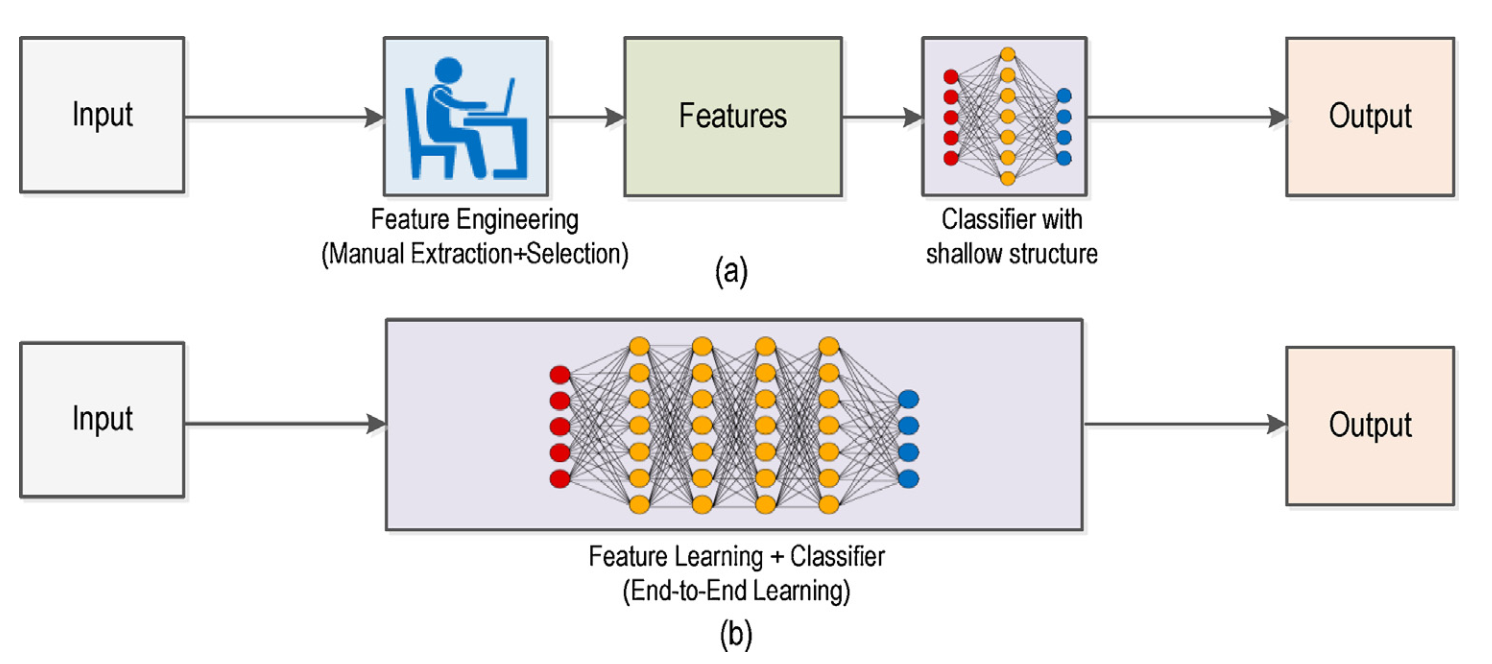
\includegraphics[width=\linewidth]{Sources/Figures/comparison.png}
%     \caption{Comparison of: (a) Traditional approach and (b) Deep learning approach. Adapted from \cite{comparison_illustration}. \todo{Zmenit obrazek, clovek mate.}}
%     \label{fig:comparison}
% \end{figure}

\subsection{Evaluation Metrics}
Firstly, let us define evaluation metrics for binary classification. Consider two classes we want to predict: \bld{positive (P)} and \bld{negative (N)}. Let
\begin{itemize}
    \item \bld{true positives (TP)} be correctly predicted P cases,
    \item \bld{true negatives (TN)} be correctly predicted N cases,
    \item \bld{false negatives (FN)} be all P cases we wrongly predicted as N,
    \item \bld{false positives (FP)} be all N cases we wrongly predicted as P.
\end{itemize}
Suppose we want to focus on the performance of P cases prediction. We define metrics \bld{precision} and \bld{recall} as follows:
$$
    \text{precision} = \frac{\text{TP}}{\text{TP} + \text{FP}}, \\
    \text{recall} = \frac{\text{TP}}{\text{TP} + \text{FN}}.
$$
Precision is also known as a positive predictive value, i.e., how many of the positive predictions (TP + FP) actually belong to P class. Recall is known as a true positive rate and it measures how many TP we have predicted out of all actual P cases (TP + FN). There is a trade-off relationship between these metrics. If we increase the precision (e.g., by setting more strict constraints for assigning TP to a prediction), the recall decreases as there would be more FN cases, and vice versa. 

For an object detection model evaluation, we can suppose that TP represents correctly detected object. Similarly, FP can be viewed as a wrongly detected object or duplicate detection. We would like to combine the precision and recall to a single composite score -- \bld{mean average precision (mAP)}. However, before we delve into its definition, let us first describe how to determine the TP and FP from the model's predictions.

\begin{figure}[H]
    \centering
    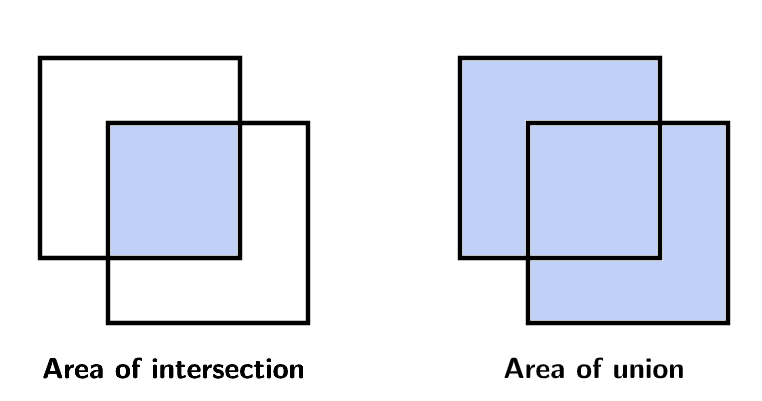
\includegraphics[width=0.6\linewidth]{Sources/Figures/iou.png}
    \caption{Illustration of two bounding boxes and the two types of areas they form.}
    \label{fig:iou}
\end{figure}

Models output a list of predictions that are defined by \bld{bounding box} coordinates (the boundaries of the detected object), \bld{predicted class}, and \bld{confidence score} of the prediction. To determine if the detection is correct, we need to define \bld{Intersubsection-over-Union (IoU)}. IoU is defined as a proportion of the area of intersubsection (overlap between predicted bounding box and the ground-truth bounding box) and the area of union (see Figure \ref{fig:iou}):
$$
    \text{IoU} = \frac{\text{area of intersubsection}}{\text{area of union}}.
$$
We simply declare the prediction as a TP if the IoU of the ground-truth bounding box and the predicted bounding box is greater than a fixed IoU threshold. Otherwise the prediction is considered as a FP. Now that we know how to determine the TP and FP cases, we can define mAP.

Mean average precision is an averaged \bld{average precision (AP)} over all classes. Let us define AP for some class $c$. We denote it as AP$_{c}$. For illustration, consider a simplified example: we collect all predictions for the class $c$ from all test images, and we rank them by the confidence score. Let \bld{positive predictions} be those predictions that have IoU > 0.5. If there are more positive predictions for a single object, only the prediction with a higher confidence score is considered to be a TP. See the example Table \ref{tab:ap}. In the definition of AP, precision is defined as the proportion of all predictions above the rank which are TP. Whereas recall is defined as the proportion of TP ranked above a given rank and all positive predictions.
\begin{table}[H]
\centering 
\begin{threeparttable}
\begin{tabular}{|c|c|c|c|c|c|}
\hline
\bld{rank} & \bld{IoU > 0.5} & \bld{confidence score} & \bld{TP/FP} & \bld{Precision} & \bld{Recall} \\
\hline
1 & yes & 98 \% & TP     & 1.00  & 0.2  \\
2 & yes & 88 \% & FP$^*$  & 0.50  & 0.2 \\
3 & yes & 78 \% & TP     & 0.67  & 0.4  \\
4 & yes & 75 \% & TP     & 0.75  & 0.6  \\
5 & no  & 60 \% & FP     & 0.60  & 0.6  \\
6 & yes & 59 \% & TP     & 0.67  & 0.8  \\
\hline
\end{tabular}
\begin{tablenotes}
      \small
      \item  $^*$ consider this example as a duplicate of the rank 1 example.
\end{tablenotes}
\caption{An example of predictions.}
\label{tab:ap}
\end{threeparttable}
\end{table}

Let us explain the calculation behind the third row. The precision is $2/3 \doteq 0.67$, because there are 2 TP out of 3 predictions above the third row (including the row). The recall is $2/5 = 0.4$, since there are 2 TP out of 5 positive predictions (IoU > 0.5). As we can see, the precision has a "zigzag" pattern as we go down the ranking. Whereas the recall is increasing. 

The AP$_c$ is defined as an \bld{area under the precision-recall curve} (see Figure \ref{fig:precisionrecall}). To reduce the impact of the zigzags, we interpolate the curve at each recall value $r$ by taking the maximum precision $p_\text{interp}$ measured "to the right":
$$
p_\text{interp}(r) = \max\limits_{\hat{r}:\hat{r} \geq r} p(\hat{r}),
$$
where $p(\hat{r})$ is the measured precision at the measured recall $\hat{r}$. We obtain a monotonically decreasing curve that can be numerically integrated as it is a piecewise constant (see the red dashed curve in Figure \ref{fig:precisionrecall}). We sample all unique recall values $R$ and compute AP$_c$ as a sum of rectangular blocks as follows:
$$
\text{AP}_c = \sum\limits^{\lvert R\rvert - 1}_{n = 0} (r_{n+1} - r_n) \cdot p_\text{interp}(r_{n+1}).
$$

\begin{figure}[H]
    \centering
    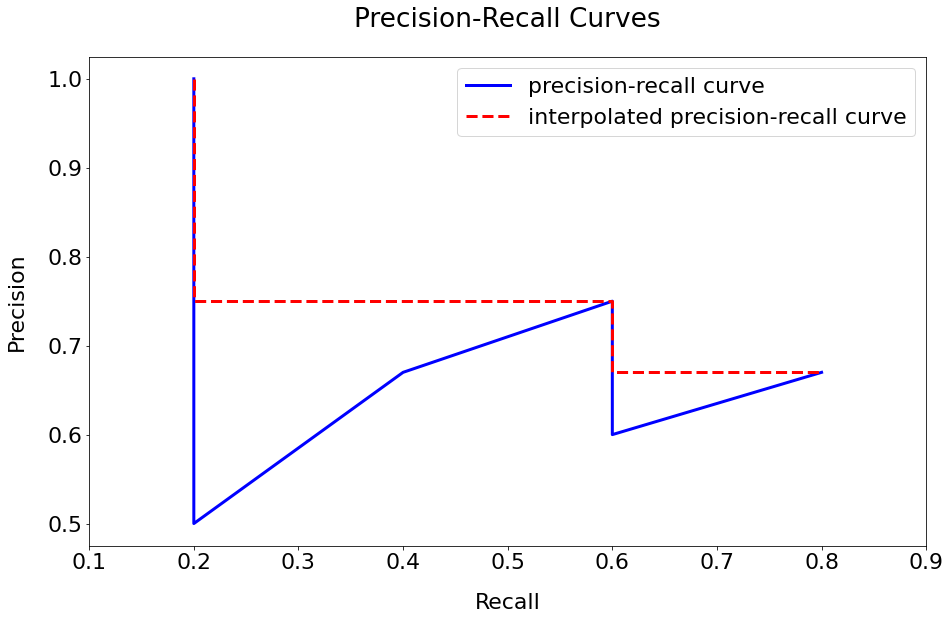
\includegraphics[width=0.8\linewidth]{Sources/Figures/precisionrecall.png}
    \caption{Precision-recall curves.}
    \label{fig:precisionrecall}
\end{figure}

We then get the final mAP by averaging all AP$_c$ for every class (let $C$ be the set of all classes):
$$
    \text{mAP} = \frac{1}{\lvert C \rvert} \cdot \sum_{ c\in C} \text{AP}_c.
$$
The VOC competitions \cite{voc} used this metric for a fixed IoU = 0.5 threshold. However, for our evaluation, we use the \bld{updated COCO challenge metric} \cite{coco} that averages the mAP over 10~different IoU thresholds (from 0.50 to 0.95 with 0.05 step size). We denote it as AP$_{.50:.05:.90}$ = AP. Similarly, for single IoU thresholds we have AP$_{50}$ (the standard VOC metric) and AP$_{75}$ (a~strict metric). They also define AP$_\text{small}$, AP$_\text{medium}$, and AP$_\text{large}$ for varying object's size:
\begin{itemize}
    \item AP$_\text{small}$ is an AP for small objects (bounding box area < $32^2$ px),
    \item AP$_\text{medium}$ is an AP for medium objects ($32^2$ px < area < $96^2$ px),
    \item AP$_\text{large}$ is an AP for large objects (area > $96^2$ px).
\end{itemize}
Note that they do not make distinction between mAP and AP. Henceforth, whenever we refer to the AP, we mean the primary COCO metric AP$_{.50:.05:.90}$. 

%%%%%%%%%%%%%%%%%%%%%%%%%%%%%%%%%%%%%%%%%%%%%%%%%%%%%%%%%%%%%%%%%%%%%%%%
\section{Deep Learning}\label{deep_learning_chapter}
%%%%%%%%%%%%%%%%%%%%%%%%%%%%%%%%%%%%%%%%%%%%%%%%%%%%%%%%%%%%%%%%%%%%%%%%

% Neural networks since 60s
% Deep learning since 2006
% Definition
  % Multiple layers
  % Based on ANN
% Impact

In this part, we briefly introduce relevant topics of deep learning. For the sake of readability, we only limit ourselves to high-level and simple descriptions. The covered concepts are very well described in the book written by the pioneers of deep learning, Ian Goodfellow, Yoshua Bengio, and Aaron Courville \cite{Goodfellow-et-al-2016}. In fact, we draw inspiration from the book for some of our definitions.

The history of artificial neural networks (ANNs) can be dated back to the 1940s \cite{McCulloch_1943}. However, only since 2006, deep architectures of ANN have become a trendy area of machine learning research \cite{DBLP:journals/corr/Schmidhuber14}. That year, Hinton et al. introduced unsupervised pre-training of deep feedforward neural networks \cite{hinton2006reducing}. Using this method on a deep belief network \cite{DBN}, the model achieved 1.2\% error rate on the MNIST classification dataset \cite{hinton2006fast, mnist}. This exceptional result drew attention to deep neural networks. The detailed historical development of artificial neural networks and deep learning is nicely overviewed in a journal article by another important figure in the field Juergen Schmidhuber 
\cite{DBLP:journals/corr/Schmidhuber14}.

\subsection{Deep Feedforward Network}
% Firstly, let us define the field of deep learning. Many of closely related definitions are summarized in \cite{mic_definitions}. We cite the one that best suits the nature of this work.  
    
% \theoremstyle{definition}
% \newtheorem*{definition}{Definition}
% \begin{definition}
% A class of machine learning techniques that exploit \textbf{many} layers of non-linear information processing for supervised or unsupervised feature extraction and transformation, and for pattern analysis and classification.
% \end{definition}

% In our case, the deep learning technique will be used for object detection, which also consists of the classification task. The selected object detection models are deep architectures of \textbf{convolutional neural network (CNN)}, which are particularly effective for image processing tasks. In the coming section, we will briefly describe the foundations of CNNs. 
The fundamental model of deep learning is a \bld{deep feedforward network}, also known as feedforward neural networks, or multilayer perceptrons. Feedforward networks approximate arbitrary functions of the form $y = f^*(x;\theta)$, where $y$ is the \bld{output}, $x$ is the \bld{input}, and $\theta$ are the network's \bld{weights} (or parameters). For example, in our case, we would like to output the list of objects with their respective coordinates and classes based on the input image. The process of finding the best weights $\theta$ for accurate approximation is called \bld{training} (or the network \bld{learns}). We describe this process in detail in Section \ref{sec:training}.

The network $f^*$ is composed of intermediate computations that are defined by some function $f^{(i)}$. We might write the approximated function as a function composition of $n$ functions: 
$$
f^*(x) = (f^{(n)} \circ f^{(n-1)} \circ ... \circ f^{(2)} \circ f^{(1)})(x).
$$
As we can see, the information flows sequentially in the network; thus, it is called feedforward. Each of the function $f^{(i)}$ is called \bld{layer}. The deep learning models are composed of many different layers. We say that the network is deep; hence, the name \bld{deep learning}. In the next sections, we describe different types of layers.



\subsection{Convolutional Neural Network}
In the following subsections we describe the layers of \bld{convolutional neural networks} that are a special case of a feedforward networks. They thrive at image processing tasks as a result of a very effective way of feature extraction.

\subsubsection{Fully-connected Layer}
The most basic layer is \textbf{fully-connected layer} (also known as \textbf{linear} or \textbf{dense} layer). It performs a transformation from \textbf{input vector} $\boldsymbol{x}$ of size $m$ into \textbf{output vector} $\boldsymbol{y}$ of size $n$. The transformation has two parameters, a \textbf{weight matrix} $\boldsymbol{W}$ of size $m \times n$ and \textbf{bias} $\boldsymbol{b}$ of size $n$. Firstly, the input vector is weighted by $W$, then the bias is added, and finally an \textbf{activation function} $\boldsymbol{f}$ is applied to every element (see Section \ref{afunctions} for more details on activation functions).
$$
y = f(W\cdot x + b)
$$
See figure \ref{fig:fcl} for a graph representation of a neural network composed of two fully-connected layers, where each node is a neuron, and each directed edge is a weight.

\begin{figure}[h]
    \centering
    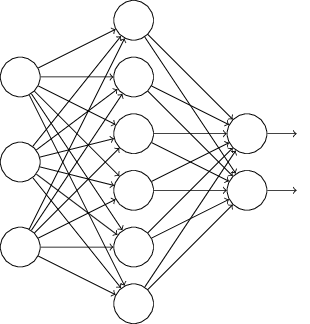
\includegraphics[width=4cm]{Sources/Figures/fully_connected_layer.png}
    \caption{Multilayer Perceptron with two fully-connected layers. Taken from \cite{nielsenneural}.}
    \label{fig:fcl}
\end{figure}

\subsubsection{Convolution Layer}
The most important layer of CNNs is the \textbf{convolution layer}. It introduces a new concept of shared weights, which help us train deeper architectures and is more suited for image processing tasks. To illustrate the convolution layer, imagine the input as a square of neurons, i.e., a two-dimensional \textbf{image} $\boldsymbol{I: (W, H) \rightarrow \real}$\todo{Zmatecna definice. Sjednotit styl notaci.}, where ${W}$ is the width and ${H}$ is the height of the image. 

In contrast with a fully-connected layer, we do not connect every input neuron to every output neuron. Instead, every output neuron is associated with a smaller region in the input image. Each association is defined by its \textbf{bias} $\boldsymbol{b}$ and $\textbf{weights}$ $\boldsymbol{K:(K_w, K_h) \rightarrow \real}$, where $K_w$, $K_h$ is the region's width and height. The output of the layer is a downscaled image $\boldsymbol{Y:(W - K_w + 1,}$ $\boldsymbol{H - K_h + 1)  \rightarrow \real}$, which is often called a \textbf{feature map}. The value of the $i, j$-th output neuron $Y(i,j)$ is defined by: 
$$
Y(i, j) = f\left((I * K)(i,j) + b\right)
$$

The $*$ operation is called \textbf{convolution}\todo{Fskutecnosti cross-correlation. Doplnit poznamku.} and is defined as follows:

$$
(I * K)(x, y) = \sum\limits_{k = 1}^{K_w}\sum\limits_{l = 1}^{K_h} I(x + k, y + l) \cdot K(k, l)
$$

This process is applied to the whole input image (see figure \ref{fig:convolution}). The convenience of this method comes with using the same weights $K$ for each convolution operation. The weights $K$ (and also bias $b$) are called \textbf{kernel} or \textbf{filter}. The kernel is trained to detect some non-linear pattern. Therefore, we use multiple kernels to recognize various features in the image (we end up with multiple feature maps). The approach also helps CNNs to adapt to image \textbf{translation invariance}, i.e., the detected features do not depend on their positions in the input image.

For illustration purpose, we have considered a two-dimensional inputs. However, in practice, we often work with RGB or even RGB-D images represented by \textbf{tensors} of shape $(W, H, C)$, where $C$ is number of channels (e.g. three for classic RGB image). 

Another important parameter of the layer is \textbf{stride length}. It defines the number of pixels the filters shifts over the input image. The bigger is stride length the more downscaled the output image is.


\begin{figure}[h]
    \centering
    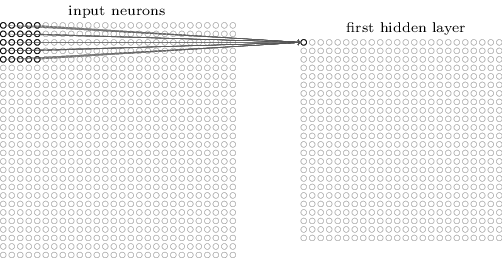
\includegraphics[width=10cm]{Sources/Figures/convolution.png}
    \caption{Illustration of a convolution layer with 5 $\times$ 5 kernel. Taken from \cite{nielsenneural}.}
    \label{fig:convolution}
\end{figure}

\subsubsection{Pooling Layer}
Another essential layer for CNNs is the \textbf{pooling layer}. In CNN architectures, the pooling layers typically come after the convolution layers. They are used for downscaling the feature maps to reduce the number of network parameters. 

The layer works in a similar manner to the convolution layer. It takes multiple values from a pooling region and outputs a single pixel. The most common type of a~ pooling operation is \textbf{max pooling}, which outputs the region's maximum value. Another operation that can be applied to the region is \textbf{average pooling}, which outputs the region's mean value.

The pooling region's shape is typically 2 $\times$ 2. In some cases, we want to pool from the whole input. We call these operations \textbf{global poolings} (e.g., global max pooling).

\subsubsection{Activation Functions}
\label{afunctions}

Activation functions introduce non-linearity to the layers. Some of the most important ones are listed below:
\begin{itemize}
\item \textbf{ReLU} (rectified linear unit) is the most popular activation function, which was introduced in \cite{pmlr-v15-glorot11a}. It is defined as follows: $\text{ReLU}(x) = \max(0, x)$. It deals better with vanishing gradient than sigmoidal functions, which tend to saturates on extreme values.
\item \textbf{Leaky ReLU} deals with the so-called \textbf{dying ReLU problem}. If we use simple ReLU, many neurons cannot recover from being stuck at zero value. We can tackle the problem by "leaking out" the negative values. The leaked values are then weighted by parameter $\alpha$: $\text{Leaky ReLU}(x) = \max(\alpha x, x)$
\item \textbf{Softmax} funciton is typically used in a last layer of classification neural networks. It takes a vector of real numbers and normalizes the values into a probability distribution. For input vector $x \in \real^K$ and output vector $y \in \real^K$, the function is defined as follows:
$$
    y_i = \text{softmax}(x)_i = \frac{e^{x_i}}{\sum\limits^{K}_{j = 1} e^{x_j}} \text{ for } i = 1,...,K
$$
\end{itemize}

\subsection{Training}
\label{sec:training}\todo{Doplnit trenovani}
\begin{itemize}
    \item Optimization task
    \item Gradient descent
    \item Backpropagation
    \item Adam, etc.
\end{itemize}
We find the best weights by minimizing the loss function $\mathcal{L}(x)$ that determines the quality of the model. There are many different loss functions. However, we describe the most common ones for classification and regression tasks.



\subsection{Overfitting and underfitting}

When we train a machine learning model, we typically have a \textbf{training set} and a \textbf{test set}. We then fit the model's parameters on a training set to \textbf{minimize} an error measure (a \textbf{training loss} or \textbf{error}). However, at the same time, we want to minimize a \textbf{test error} as well. We say that a model should \textbf{generalize}. This means that it should perform well on unseen data.

These efforts can lead to two major problems in machine learning. If we train for too long, the model will learn the training set patterns that do not generalize to the test set. We say that the model \textbf{overfits}. The opposite of overfitting is \textbf{underfitting}. It occurs when the model is not able to gain sufficiently low training loss. Underfitting can happen because of using a weak model or not training long enough. If we plot the losses, we want to make sure that the training loss is reasonably low, and the gap between training and test error is small (see figure \ref{fig:loss_plot}).
 
\begin{figure}[h]
    \centering
    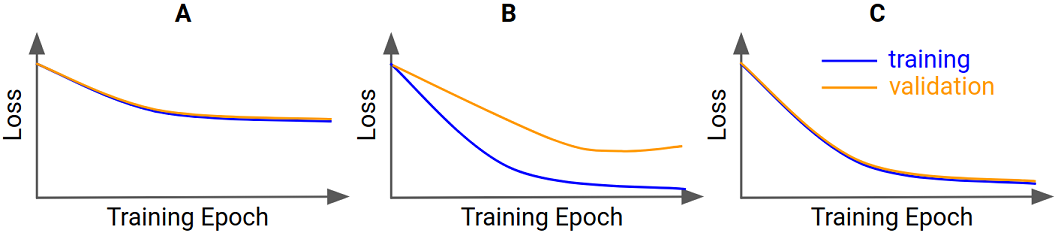
\includegraphics[width=\linewidth]{Sources/Figures/fitting.png}
    \caption{A simplified cases of loss curves \protect\footnotemark showing: (A) Underfitting, (B) Overfitting and (C) Optimal fit. Taken from \cite{bileschi2020deep}.}
    \label{fig:loss_plot}
\end{figure}

\footnotetext{The terms validation and test set are sometimes used interchangeably. However, the true meaning is not important for the illustration. Both are unobserved data.}

In coming subsections we describe the most common techniques to prevent overfitting in neural networks.
\footnotetext[2]{The simplest explanation is most likely the right one.}
\subsubsection{$L_2$ Regularization}
Following the Occam's razor principle\footnotemark , the extreme weights are likely to cause overfitting. We can reduce the overfitting by penalizing these weights with $\boldsymbol{L_2}$ \textbf{regularization}. The penalization is performed by adding a $L_2$ term to the loss function. The term is defined as a sum of squares of weight values. 



\subsubsection{Dropout}
Another common technique is called \textbf{dropout}. This method prevents individual nodes in the network to rely on the output of other nodes by randomly "dropping out" or "deactivating" some of the neurons. The method's parameter is a number between 0 and 1 that defines the fraction of the input units to drop.

\subsubsection{Batch Normalization}
Deep neural networks often suffer from unstability. Small changes in layers close to the input amplify as they propagate through the network. The deeper layers have to adapt significantly and thus learn slowly. \textbf{Batch normalization} introduces a way to stabilize and accelerate the training speed by normalizing the outputs of previous layer by subtracting the batch mean and dividing by the batch standard deviation.

\subsubsection{Data Augmentation}
The most obvious way to train a robust model is to have an extensive dataset. However, in some cases, it is very challenging to acquire sufficient ammount of data. We can overcome this issue by 
\textbf{augmenting} the training set by generating new artificial data. Of course, it is impossible to adopt this approach to every type of datasets, but it is straightforward for object detection tasks. The simplest way to augment the image dataset is by adding \textbf{random transformations} (cropping, resizing, rotation, ...) of the original images. The more sophisticated method would be generating new \textbf{synthetic} images. With recent advances in generative adversarial networks (GANs), it is possible to synthesize high-quality images. An impressive adoption of this approach is proposed in \cite{wei2019generative}.














\chapter{Models}
The first deep learning-based object detection models emerged after a breakthrough in ImageNet Large Scale Visual Recognition Challenge (ILSVRC) \cite{ILSVRC15} in 2012 when Alex Krizhevesky et al. proposed a deep and wide CNN classification model . The so-called AlexNet outperformed traditional state-of-the-art models.  This architecture was later exploited as a feature extractor for the CNN-based object detection model R-CNN \cite{rcnn}, which also surpassed the previous best results on PASCAL Visual Object Classes (PASCAL VOC) dataset 2012 \cite{voc}. Since then, many CNN-based object detection models were introduced \cite{odreview}.

Generally, they can be categorized into two types: one-stage detectors and two-stage detectors. The latter approach consists of a region proposal step, followed by classification and bounding box regression. This means that the model initially generates interesting regions, which are then analyzed one-by-one. In contrast, one-stage detectors are based on a global regression and classification, requiring a single pass through the network, and thus they are usually faster but less accurate. A common property of both approaches is that we can easily substitute the models' feature extractor. 

For our comparison, we have chosen three state-of-the-art models: Faster R-CNN \cite{fasterrcnn}, Cascade R-CNN \cite{cascadercnn}, and RetinaNet \cite{retinanet}. The first one was proposed in 2015, and it is a well-known example of two-stage detectors. The model is considered to be well-established as it has a reasonable accuracy/speed trade-off and is easy to modify. In our work, Faster R-CNN serves as a baseline for our comparison. The next one, Cascade R-CNN, is an extension to Faster R-CNN, which improves the performance by addressing some of its caveats. Finally, RetinaNet is a recent one-stage detector introduced by the Facebook AI Research team (FAIR), aiming to match the two-stage detectors' accuracy while preserving one-stage detectors' speed. We describe all these models in detail in the following sections.

\section{Architecture}
The architecture of models can be divided into two parts: backbone and detection head. The backbone is responsible for computing feature maps from the input image. The feature maps are then used for predicting the bounding boxes and classifications by the detection head. All our models use ResNet \cite{resnet} as a backbone. Except for the Faster R-CNN's backbone, the ResNet is additionally extended with Feature Pyramid Network (FPN) \cite{fpn}, which helps with detecting objects at different scales. We describe ResNet, FPN, and each model's detection head in the following sections.

\section{ResNet}
Deeper neural network architectures are harder to train because of the disappearing gradient. As the gradient is backpropagated through the network, the repeated multiplication by values between 0 and 1 makes the gradient very small, and eventually, it vanishes. Thus the earlier layers (closer to the input) are not trained properly. This is called the vanishing gradient problem. 

ResNet is a CNN-based image recognition model proposed in 2015 in \cite{resnet} to solve the difficulties of training deeper architectures by introducing skip connections between the layers allowing to train up to 1001-layer deep architectures. For comparison, the previous state-of-the-art model VGG \cite{vgg} consists of up to 19 sequentially stacked layers (see Figure \ref{fig:vgg_resnet}).

\begin{figure}[h]
    \centering
    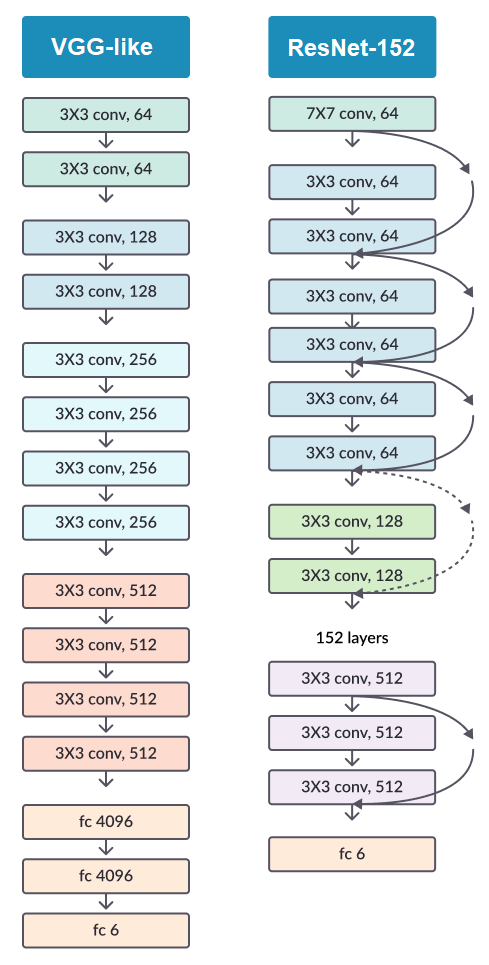
\includegraphics[width=0.4\linewidth]{Sources/Figures/vgg_resnet.png}
    \caption{A visual comparison of a VGG-like network and ResNet.}
    \label{fig:vgg_resnet}
\end{figure}

Skip connections are realized by performing identity mapping. Its outputs are then simply added to the outputs of the stacked layers (see Figure \ref{fig:residual_block}). This helps with propagating the gradient deeper in the network. 

\begin{figure}[h]
    \centering
    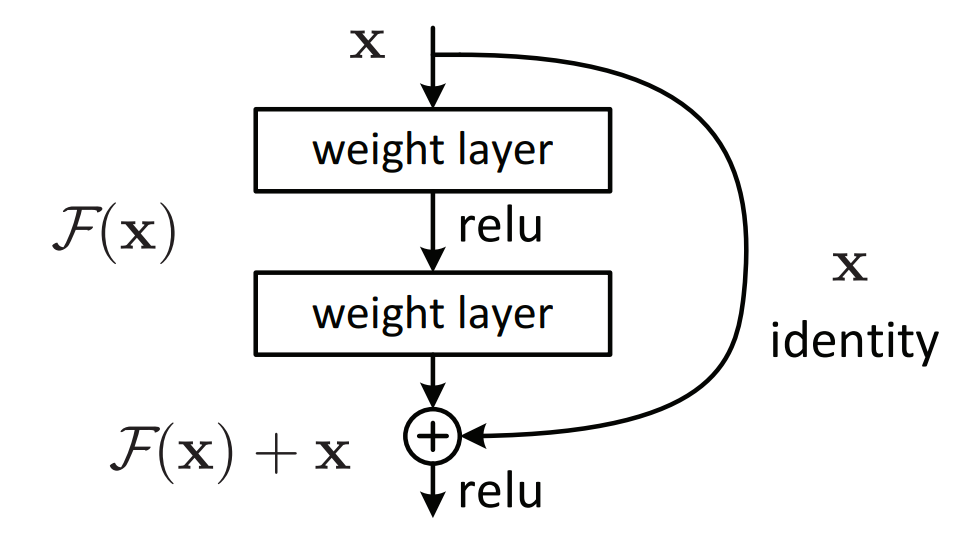
\includegraphics[width=0.4\linewidth]{Sources/Figures/residual_block.png}
    \caption{Visualization of a skip connection.}
    \label{fig:residual_block}
\end{figure}

\section{Feature Pyramid Network}
One of the challenges of object detectors is to detect objects at different scales. To approach this, we can simply process the same image at different scales. However, this naive method is very inefficient and requires a lot of computation time and memory. A more efficient way would be to take the computed feature maps that are already of different scales and use them for the prediction. But the feature maps closer to the input are composed of low-level features (e.g., edges), which are not very valuable for accurate predictions. We can visualize these approaches as a pyramid of images or features (see Figure \ref{fig:pyramids}). 

\begin{figure}[h]
    \centering
    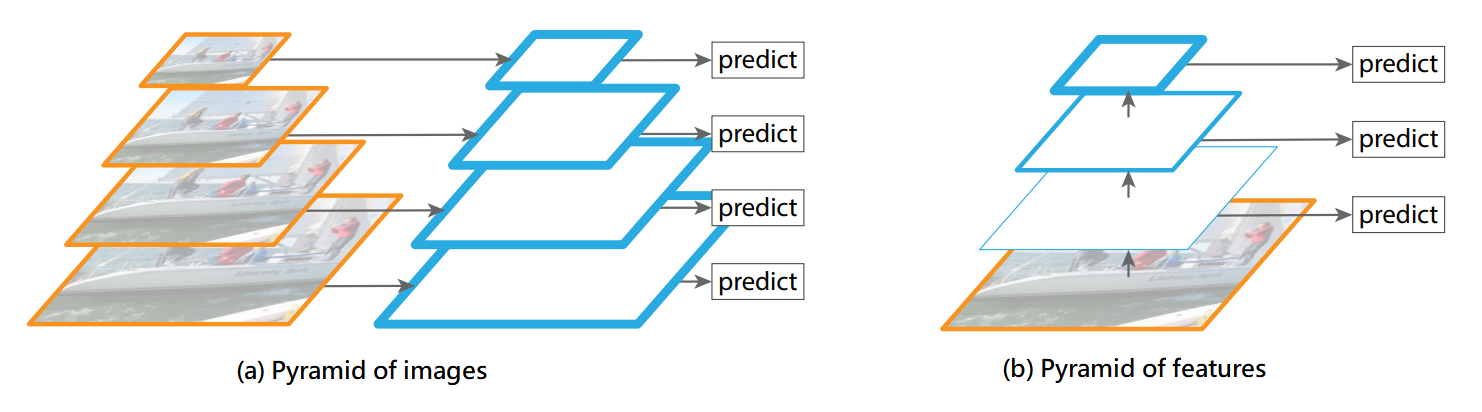
\includegraphics[width=\linewidth]{Sources/Figures/pyramids.png}
    \caption{(a) Features are computed independently for each scale; (b) exploits the computed feature maps of feature extractor. Adapted from \cite{fpn}}
    \label{fig:pyramids}
\end{figure}

In 2017 Lin et al. proposed Feature Pyramid Network \cite{fpn}. The network enhances the feature maps from lower pyramid levels with high-level features. To achieve this, the construction of the feature pyramid involves a bottom-up pathway and a top-down pathway (see Figure \ref{fig:fpn}). The bottom-up pathway is a conventional CNN feature extractor, which gradually produces smaller and smaller feature maps, but with high-level features (we say that they are semantically richer). The top-down pathway upsamples the semantically richer features to match the higher resolution of the bottom-up pathway feature maps. These different feature maps are then added together via lateral connections between them. Those connections also help to make training easier, similarly as in ResNet.  Finally, these semantically enriched multi-scale feature maps can be used by the detection head of an object detection model. 

\begin{figure}[h]
    \centering
    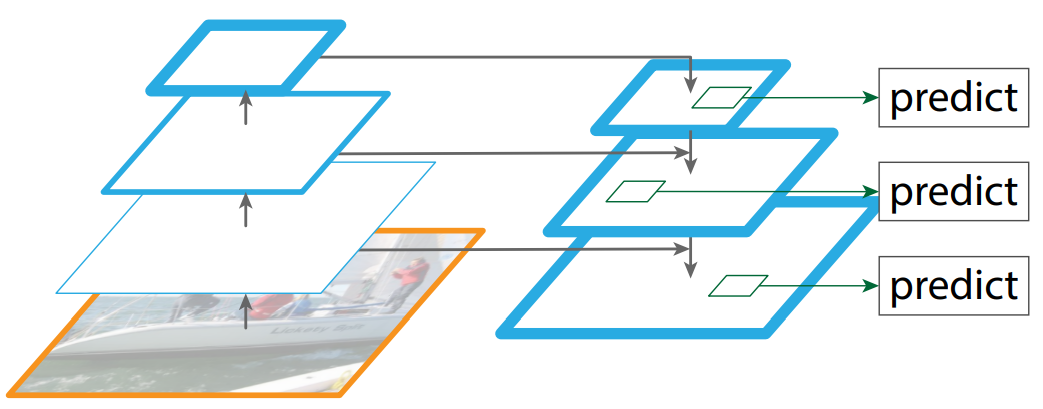
\includegraphics[width=0.6\linewidth]{Sources/Figures/fpn.png}
    \caption{FPN with bottom-up pathway (left), top-down pathway (right) and lateral connections (horizontal arrows) \cite{fpn}.}
    \label{fig:fpn}
\end{figure}

\section{Faster R-CNN}
The first model we describe is Faster R-CNN proposed in 2015 by the same co-authors of ResNet \cite{fasterrcnn}. As we mentioned at the beginning of the chapter, Faster R-CNN is a two-stage detector. Firstly, it generates candidate regions of interest (RoIs or proposals). This step is known as a region proposal. The regions are then processed in the detection head that outputs the predicted category and the bounding box's coordinates.  For a high-level description, we visualize the model with a network flow graph as in Figure \ref{fig:fasterrcnn}. 

\begin{figure}[h]
    \centering
    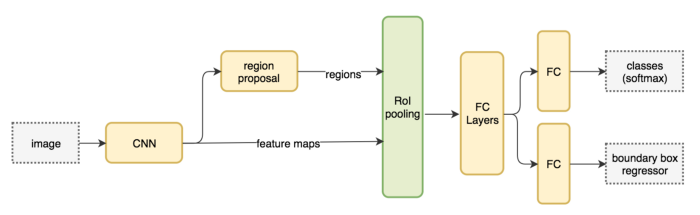
\includegraphics[width=\linewidth]{Sources/Figures/fasterrcnn.png}
    \caption{High-level Faster R-CNN flow. FC stands for fully-connected \cite{huifasterrcnn}.}
    \label{fig:fasterrcnn}
\end{figure}

As we can see, Faster R-CNN firstly computes the feature maps, which are then exploited by two separate computational branches. The region proposal is carried out by a Region Proposal Network (RPN). The corresponding features of the proposed RoIs are retrieved from the initial feature maps by a method called RoI pooling. The proposals' feature maps are then fed to the fully-connected network responsible for the final category (class) and bounding box prediction. We describe each component in detail below.

\subsection{Region Proposal Network}\label{rpn}
A significant part of RPN's architecture resembles a standard CNN image classifier. The network does not predict the raw coordinates, but instead, it learns to predict offsets of reference boxes. We call these reference boxes anchors, and we place them on every point in the feature map (see Figure \ref{fig:rpn}). Each point has several anchors of different sizes and ratios. We predict an "objectness" score for each anchor, which is the anchor's probability of being an object. At the same time, we regress the offsets of the anchors. We determine the ground truth bounding box with a IoU threshold, i.e., if a proposal overlaps any ground truth bounding box, then it is assigned to it. Since we now have a large set of proposals that can overlap, we apply Non-Maximum Suppression (NMS) to solve the issue of duplicates. NMS is a greedy method that goes through the list of proposals sorted by score and removes proposals with an IoU larger than the predefined threshold with a proposal that has a higher score. Finally, the network outputs top $n$ proposals ($n = 2000$ in original paper).

\begin{figure}[h]
    \centering
    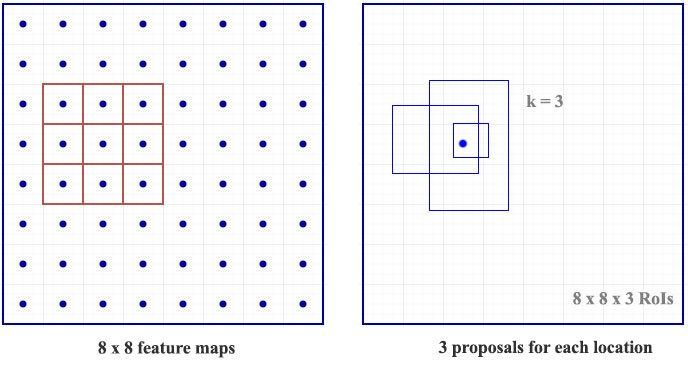
\includegraphics[width=0.6\linewidth]{Sources/Figures/rpn.jpeg}
    \caption{In this illustration, for each point we generate three proposals based on the 3 $\times$ 3 features around the point \cite{huifasterrcnn}.}
    \label{fig:rpn}
\end{figure}

\subsection{RoI Pooling}
Once we have proposals of different sizes and ratios, we need to convert maps to their corresponding features to fixed-size feature maps because the fully-connected network has a fixed-length input by definition. The conversion is done by RoI pooling layer that takes the input proposals and outputs fixed-size feature maps.  For every input proposal, crop the corresponding section in the input feature map. If we need a $w \times h$ output feature map, we equally divide the section into $w \times h$ blocks. We then apply max-pooling for these blocks, creating a new $w \times h$ feature map. For illustration, see Figure \ref{fig:roipooling}.
\begin{figure}[h]
    \centering
    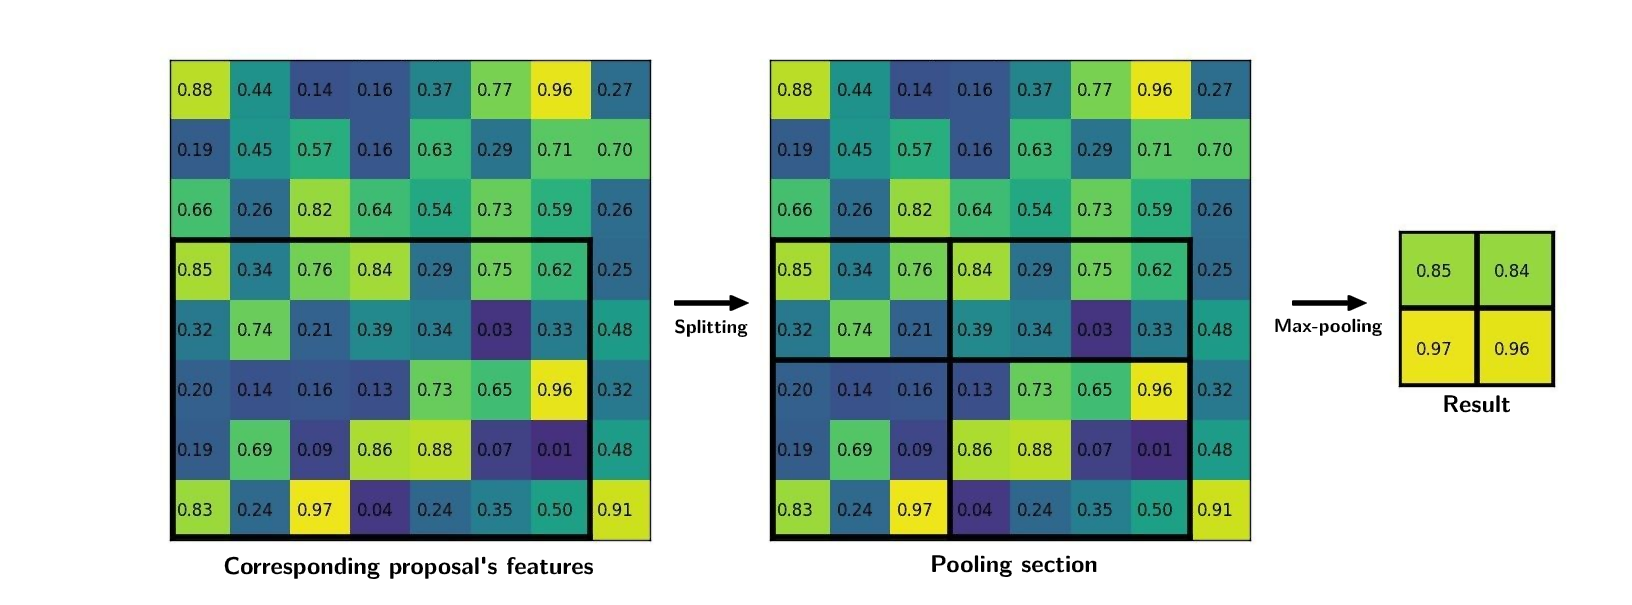
\includegraphics[width=0.9\linewidth]{Sources/Figures/roi.png}
    \caption{Illustration of RoI pooling outputting a $2\times 2$ feature map. \cite{roipooling}}
    \label{fig:roipooling}
\end{figure}

\subsection{Fully-connected Layers}
Each output of the RoI pooling layer is flattened (i.e., if we have a tensor of shape $w \times h\times channels$, we reshape it to a $w \cdot h \cdot channels$-dimensional vector) and passed into fully-connected layers. Similarly, as in RPN, these layers are responsible for adjusting the bounding box coordinates and category prediction (in RPN we only predicted if the proposal contains an object or not). The ground truth bounding boxes are determined similarly as in RPN. The IoU threshold value is usually set to 0.5. The component's architecture is visualized in Figure \ref{fig:rcnn}.
h
\begin{figure}[h]
    \centering
    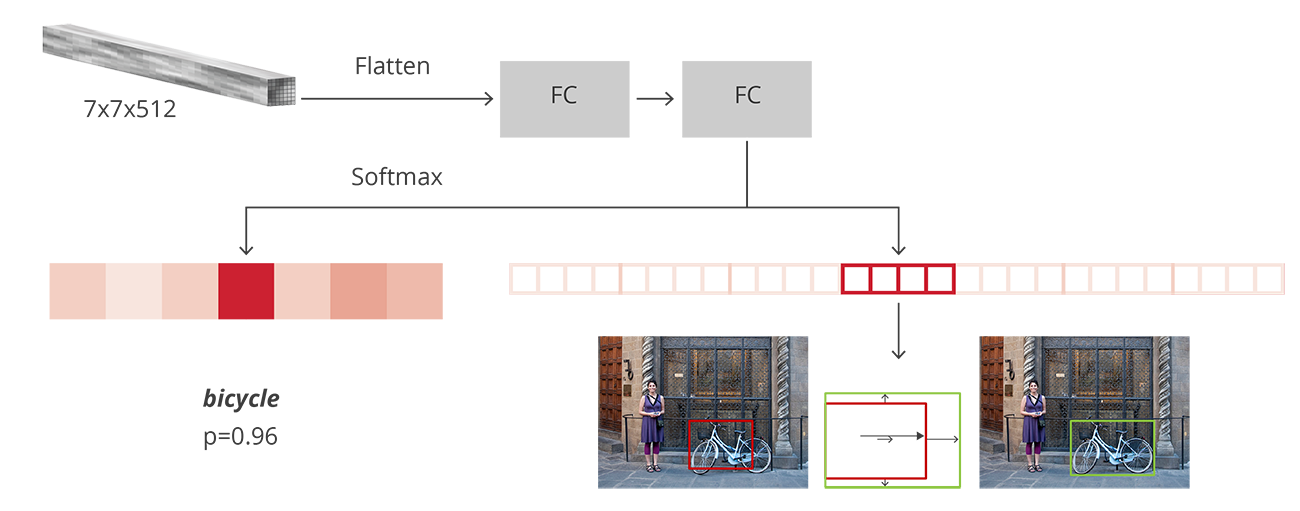
\includegraphics[width=0.8\linewidth]{Sources/Figures/rcnn-architecture.6732b9bd.png}
    \caption{Visualization of classification and regression component \cite{fasterrcnnhead}.}
    \label{fig:rcnn}
\end{figure}
 
\section{Cascade R-CNN}
As we mentioned in the previous section, Faster R-CNN is trained with a relatively small IoU threshold value. Such a low threshold value produces many noisy detections. However, setting a higher value would cause the detector to miss a lot of objects. This problem is addressed by an architecture proposed in 2017 by Cai et al. \cite{cascadercnn}. They observed that the output of a detector trained with a certain IoU threshold is a good set of proposals to train the detector of the next higher IoU threshold. The architecture extends the Faster R-CNN's detection head by adding a sequence of detection heads with increasing IoU thresholds. Since the architecture's detection part resembles a cascade (see Figure \ref{fig:cascade}), the authors call it Cascade R-CNN. This enhancement achieved better results on a COCO dataset \cite{coco} than a simple Faster R-CNN architecture.

\begin{figure}[h]
    \centering
    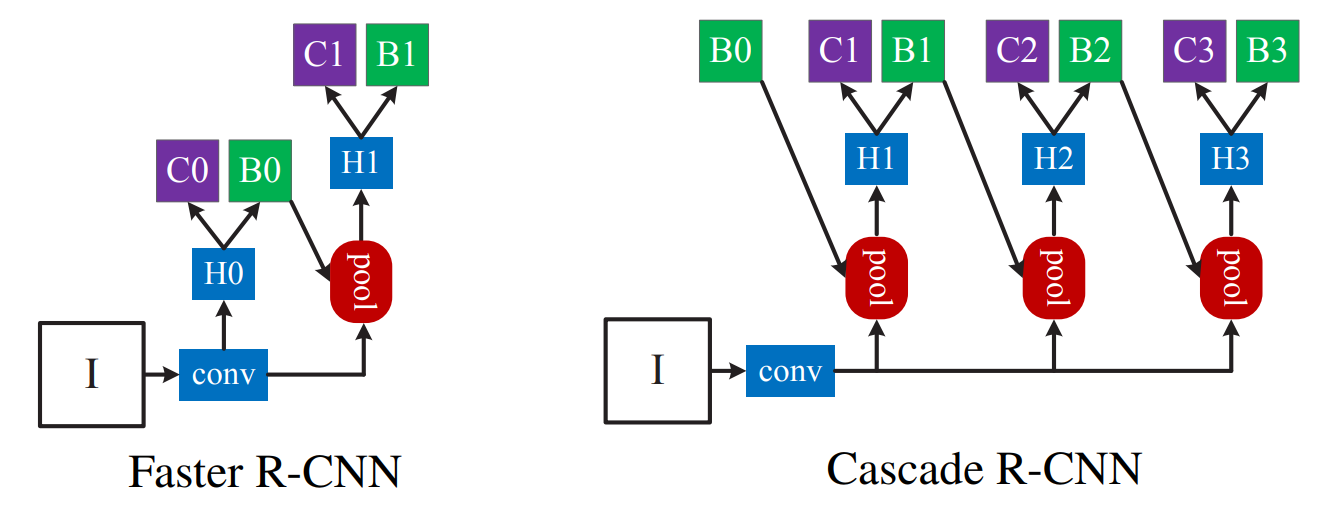
\includegraphics[width=0.7\linewidth]{Sources/Figures/cascade.png}
    \caption{Illustration of different architectures. "I" is input, "H" is fully-connected layers, "C" is classification, "B" is proposals, "conv" is backbone convolutions, "pool" is RoI pooling \cite{cascadercnn}}
    \label{fig:cascade}
\end{figure}

\section{RetinaNet}
The last model we use is a one-stage detector. One-stage detectors achieve faster inference speed than two-stage detectors by skipping the region proposal stage, predicting the bounding boxes and categories directly in a single pass. One-stage detectors tend to have worse accuracy than two-stage detectors.  However, recent proposals of new one-stage architectures achieve similar accuracy while maintaining the faster speed \cite{retinanet, yolo3}. This section covers the architecture of a detector called RetinaNet proposed by Lin et al. in 2018. 

Its architecture resembles RPN (recall Section \ref{rpn}). However, instead of predicting the objectness score, it predicts the final class. It also uses anchor boxes similar to those in RPN. The backbone of RetinaNet is based on ResNet with FPN extension. Every FPN pyramid level is then connected to two subnetworks: a class prediction subnetwork and a bounding box regression subnetwork. These subnetworks are fully-convolutional. That means they do not contain any fully-connected layers, making it possible to feed in variable inputs. See Figure \ref{fig:retinanet} for an illustration of the architecture.

\begin{figure}[h]
    \centering
    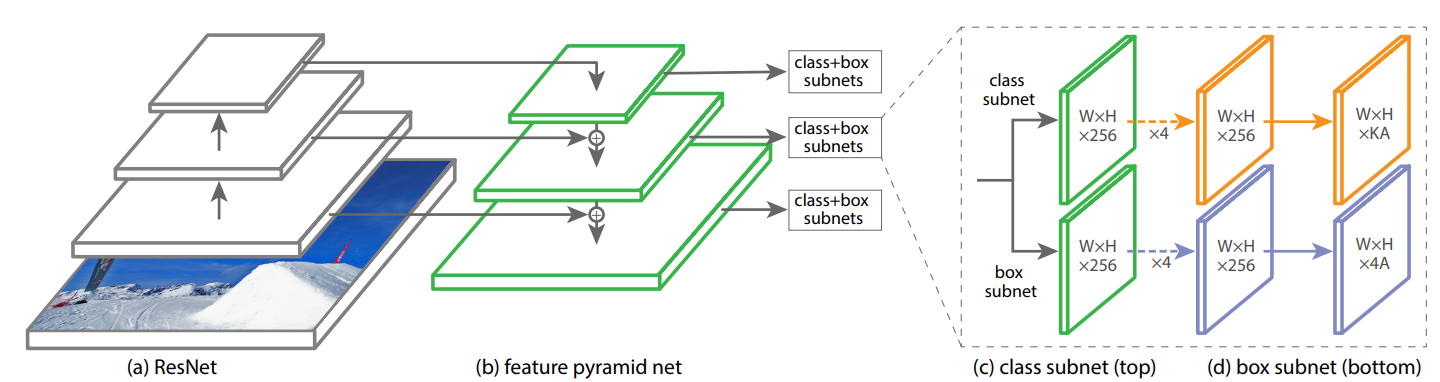
\includegraphics[width=\linewidth]{Sources/Figures/retinanet.png}
    \caption{RetinaNet's architecture. (a) and (b) form the backbone, while (c) and (d) are responsible for the class prediction and box regression \cite{retinanet}.}
    \label{fig:retinanet}
\end{figure}

RetinaNet was designed to evaluate the effectiveness of a newly proposed Focal Loss function that improves the training. The authors observed that previous one-stage detectors \cite{yolo1, yolo2, ssd} suffer from extreme foreground-background class imbalance. This means that the networks generate a vast number of anchor boxes, and the majority of them are boxes with no object in it. The authors believe this issue hurts the training as the detector is rather taught to detect the background instead of being taught to detect the actual objects.  They address this problem by reshaping the standard cross-entropy loss, so it down-weights the loss assigned to well-classified examples, since most of those examples are just the background examples.

For simplicity, lets consider a cross-entropy (CE) loss for binary classification:
\[ 
\text{CE}(p, y) = \left\{
\begin{array}{ll}
    -\log(p)   & \text{if } y = 1 \\
    -\log(1-p) & \text{otherwise.} \\
\end{array} 
\right. 
\]
Where $y = {-1, 1}$ representing the ground-truth class and $p \in [0, 1]$ is the model's estimated probability for the class $y = 1$. For convenience, we define $p_t$:
\[ 
p_t = \left\{
\begin{array}{ll}
    p   & \text{if } y = 1 \\
    1-p & \text{otherwise.} \\
\end{array} 
\right. 
\]
We then simplify $\text{CE}(p,y) = \text{CE}(p_t) = -\log(p_t)$. The CE loss is reshaped by adding a modulating factor $(1 - p_t)^\gamma$. The $\gamma \geq 0$ is a tunable parameter. Finally, we have:
$$
    \text{FL}(p_t) = (1-p_t)^\gamma \log(p_t).
$$
Lets consider that the easily-classified examples have $p_t$ near 1. As we can see, if $p_t$ is near 1, the modulating factor decreases to 0 and down-weights the loss (see Figure \ref{fig:focalloss} with various values for $\gamma$).

\begin{figure}[h]
    \centering
    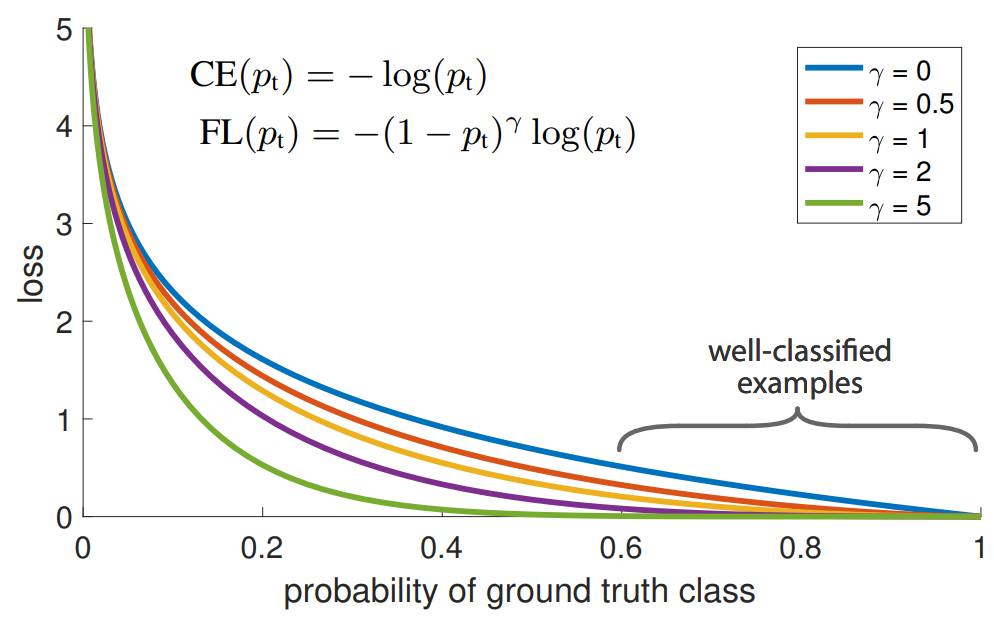
\includegraphics[width=0.7\linewidth]{Sources/Figures/focalloss.png}
    \caption{The focal loss down-weights the loss for well-classified examples. If we set $\gamma$ to 0, we get the standard cross-entropy loss \cite{retinanet}.}
    \label{fig:focalloss}
\end{figure}

These improvements led to outperforming both one-stage detectors and two-stage detectors on a COCO dataset \cite{coco}.




\chapter{Evaluation}
In this chapter, we introduce the provided datasets we evaluate the models on.
We then set hypotheses about the assumed performances of the chosen models on
our datasets. Next, we describe our process of training. We briefly mention the
technologies we have used and how we have chosen our models' parameters.
Finally, we present our achieved results and discuss them.

\section{Datasets}
We are provided with three datasets by the company SANEZOO. Unfortunately, two
of the datasets cannot be published as they are protected under a
confidentiality agreement. However, we provide sufficient characteristics of the
datasets. We summarize the basic information of the datasets in Table
\ref{tab:datasets}. Detailed description is provided below the table.
\todo{Doplnit chybejici udaje.}

\begin{table}[h]
	\centering
	\begin{tabular}{|l|l|l|l|l|}
		\hline
		\bld{Type}       & \bld{Difficulty} & \bld{Size}             & \bld{Classes}          & \bld{Publishable} \\ \hline
		Candies          & Easy             & 150                    & 1                      & Yes               \\
		Metal parts      & Medium           & 5790                   & 7                      & No                \\
		Medical supplies & Hard             & \textit{bude doplneno} & \textit{bude doplneno} & No                \\ \hline
	\end{tabular}
	\caption{Datasets summary.}
	\label{tab:datasets}
\end{table}


\begin{figure}[H]

	\begin{subfigure}[c]{0.5\textwidth}
		\centering
		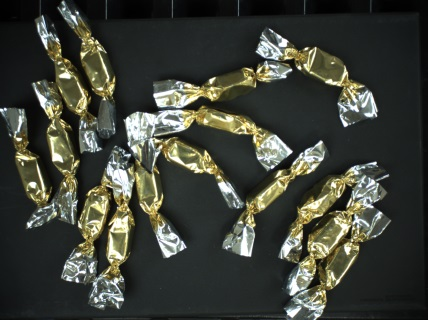
\includegraphics[width=0.9\linewidth]{Sources/Figures/sparse.jpg}
		\caption{Sparse example}

	\end{subfigure}
	\begin{subfigure}[c]{0.5\textwidth}
		\centering
		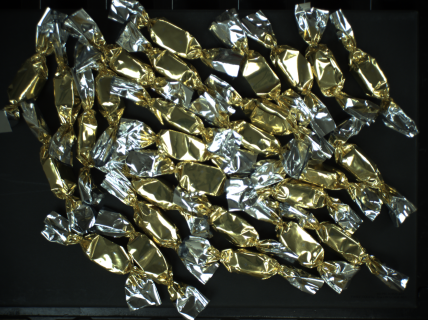
\includegraphics[width=0.9\linewidth]{Sources/Figures/dense.png}
		\caption{Dense example}

	\end{subfigure}

	\caption{Examples of candies dataset.}
	\label{fig:candies}
\end{figure}

\bld{Candies dataset.} Only the first dataset is publishable; thus, we provide a
visual example image in Figure \ref{fig:candies}. The images consist only of a
single class -- a golden candy. The density of objects (how densely they cover
the image) varies through the dataset (see Figure \ref{fig:candies}). Object
occlusions can occur in dense images; therefore, the dataset is not trivial.
However, compared to our other datasets, it is still a simpler dataset as it
strictly contains only a single class without foreign objects. Therefore, we
assign an easy difficulty to this dataset.


\bld{Metal parts dataset.} The second dataset consists of images with small
metal parts (such as shafts, rings, casings). See Figure \ref{fig:parts} for
rough illustration. The objects are placed in a plastic bin. There is always
only one class of objects on a single image. The images are taken from a
top-down perspective, similarly as in Figure \ref{fig:candies}. However, they
are taken from various angles. The density of objects also differ through the
dataset as in the first dataset (you can imagine a pile of metal parts).

\begin{figure}[ht]
	\centering
	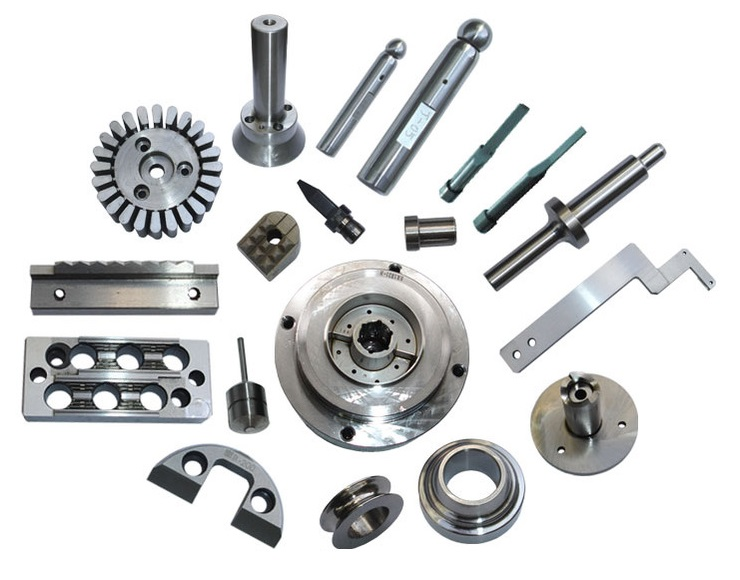
\includegraphics[height=0.35\linewidth]{Sources/Figures/metal_parts.jpg}
	\caption{An illustration of classes from metal parts dataset. Taken from
		\cite{parts}.}
	\label{fig:parts}
\end{figure}

\bld{Medical supplies dataset} The last set is made up of sequences of images
taken from an assembly line's top view. The images capture a manual assembly of
packages that are consisted of medical items (such as bandages, plastic cups, or
surgery tools). We assign a hard difficulty to this dataset because of the
non-static environment. To be more specific, the packages are in motion in some
images; therefore, the objects are slightly blurred. Moreover, occlusion of
objects occurs in the image very often since the operator does the packing
manually, and the objects are stacked on top of each other. Some objects are
tough to distinguish if they are next to each other (imagine a pile of cotton
balls). The images are taken from above the operator similarly as in the first
dataset.

\section{Hypotheses}
Let us recapitulate the models we evaluate:
\begin{itemize}
	\item Faster R-CNN with ResNet-50 backbone without FPN,
	\item Cascade R-CNN with ResNet-50 backbone with FPN,
	\item RetinaNet with ResNet-50 backbone with FPN.
\end{itemize}
We set hypotheses based on the results obtained in the models' original papers
\cite{fasterrcnn,cascadercnn,retinanet} and the \bld{Detectron2's} benchmark
results \cite{detectron}.
\renewcommand{\theenumi}{\alph{enumi}}
\begin{enumerate}
	\item Models will perform better on average on our datasets than on COCO
	      datasets \cite{coco} by a significant margin as the COCO dataset is
	      very hard.
	\item Faster R-CNN serves as a baseline and will perform the worst. Cascade
	      R-CNN should perform better than RetinaNet R-50.
	\item RetinaNet R-50 should have the fastest inference speed per image.
\end{enumerate}

\section{Training}
The models were evaluated by \bld{Detectron2} object detection framework
\cite{detectron} based on Python deep learning library \bld{PyTorch}
\cite{pytorch}. Detectron2 includes various pretrained object detection
models and tools for creating, training and evaluating of the models. We have
modified the framework's \texttt{DefaultTrainer} to meet our needs. We list
some of the modifications below:
\begin{itemize}
	\item The \texttt{DefaultTrainer} trains the model for a given number of
	      iterations (one training step of a minibatch). However, it is more
	      common to set the training for a given number of \bld{epochs}. One
	      epoch corresponds to one pass of the full training set of data. Thus,
	      the number of iterations of one epoch corresponds to fraction of the
	      training set's size to minibatch size. We have implemented this
	      simple conversion.
	\item The interval of a periodical output (\bld{checkpoint}) of the
	      training process was fixed. We have modified the behavior to output the
	      intermediate results after an arbitrary number of iterations.
	\item By default, the training process does not show the validation loss in
	      every checkpoint output. Therefore, we have implemented a
	      \texttt{ValidationLoss} hook that computes the validation loss after every
	      checkpoint's training step.
\end{itemize}
To train a model with Detectron2, we had to convert our datasets' annotations to
Detectron2's standard format.
\footnote{
	\url{https://detectron2.readthedocs.io/tutorials/datasets.html
		\#standard-dataset-dicts}
}
The format is a list of Python dictionaries.Each dictionary describes each image
and the objects included in the image. We have converted the datasets to the
appropriate format. To preserve the conversions for later use, we have exported
them  to JSON files. We have randomly split the datasets into training, test,
and validation sets by \bld{70:15:15 ratio}.

The training process is very computationally intensive and requires CUDA-enabled
GPUs.\footnote{CUDA is NVIDIA's interface for parallel computing. See
	\url{https://developer.nvidia.com/cuda-zone}} We have therefore utilized the
\bld{Google Collaboratory} (or Google
Colab) cloud service that offers limited GPU usage. Every Google Colab instance
is accessed through so-called Colab notebooks -- interactive environments that
let users add Python code cells and execute them.\footnote{
	They are in fact a cloud-hosted Jupyter Notebooks. See
	\url{https://jupyter.org/} for more details.
} The outputs of the code cells are placed below the cell after the execution.
Since the service aims mainly at users experimenting with machine learning,
there are many relevant libraries preinstalled.

Detectron2 offers pretrained detectors on the COCO dataset \cite{coco}. Each
model also contains a pretrained backbone on the ImageNet database
\cite{imagenet}. We retrain these models on our datasets by changing the number
of output classes.

We use Detectron2's predefined data augmentation for every dataset. The first
augmentation method is \texttt{ResizeShortestEdge} that scales the images while
preserving the image's aspect ratio. The second method is \texttt{RandomFlip}
that flips the image horizontally or vertically with a given probability. We
train every model with SGD with momentum and weight decay ($\mathcal{L}_2$
regularization). The learning rate is by default scheduled with
\texttt{WarmupMultiStepLR} that simply starts with a low learning rate and
increases to a defined base learning rate. We summarize the different parameters
for each model and datasets in the Table \ref{tab:parameters}.


\begin{table}[h]
	\centering
	\begin{tabular}{l|c|c|c}
		                            & Minibatch size & Learning rate & Epochs \\
		\hline
		\textit{Candies}            &                &               &        \\
		\hspace{0.1cm}Faster R-CNN  & 8              & 0.001         & 60     \\
		\hspace{0.1cm}Cascade R-CNN & 8              & 0.001         & 70     \\
		\hspace{0.1cm}RetinaNet     & 8              & 0.001         & 70     \\
		\hline
		\textit{Metal parts}        &                &               &        \\
		\hspace{0.1cm}Faster R-CNN  & 8              & 0.001         & 13     \\
		\hspace{0.1cm}Cascade R-CNN & 16             & 0.002         & 40     \\
		\hspace{0.1cm}RetinaNet     & 16             & 0.002         & 40     \\
		\hline
		\textit{Medical}            &                &               &        \\
		\hspace{0.1cm}Faster R-CNN  & 8              & 0.001         & 40     \\
		\hspace{0.1cm}Cascade R-CNN & 16             & 0.002         & 50     \\
		\hspace{0.1cm}RetinaNet     & 16             & 0.002         & 50
	\end{tabular}
	\caption{Chosen training parameters for each model.}
	\label{tab:parameters}
\end{table}
The other parameters such as model-specific parameters or optimizer parameters
are kept at default values.\footnote{Can be observed at
	\url{https://github.com/facebookresearch/detectron2/tree/master/configs} and \\
	\url{https://detectron2.readthedocs.io/modules/config.html?highlight=configs\#config-references}}
We stopped the training earlier when we observed that the model's loss was
changing only by small margins. After training we chose the best weights by
observing the value of the validation loss w.r.t. to the value of the training
loss (see Figures \ref{fig:candies_loss}, \ref{fig:metal_loss}, and
\ref{fig:medical_loss}). Generally, we were looking for the lowest validation
loss. However, if we observed an overfitting pattern, we chose earlier weights
to moderate it.
\section{Results}
We present the evaluation results in the following sections that are divided by
the datasets.

\subsection{Candies dataset}
The resulting AP metrics for the candies dataset can be seen in Table
\ref{tab:candies}. We can see that the AP is indeed higher than for the COCO
dataset (44.3 for Cascade R-CNN \cite{detectron}). Another observation we make
is that the main APs (AP, AP$_{50}$, AP$_{75}$) do not differ that much. And
in fact, they do not match with our hypothesis (b) as the Cascade R-CNN is the
worst model. We strongly believe that this is caused by small dataset size. The
test set consists only of 22 images. The random sample of test images can
greatly affect the resulting AP as the small sample may not cover most of the
cases of the images. Moreover the small training size also causes overfitting
as we can see in the Figure \ref{fig:candies_loss}.

\begin{table}[H]
	\centering
	\begin{tabular}{l|l|l|l|l|l|l}
		Model                  & AP    & AP$_{50}$ & AP$_{75}$ & AP$_\text{large}$ & AP$_\text{medium}$ & AP$_\text{small}$ \\
		\hline
		RetinaNet R-50 FPN     & 66.09 & 99.27     & 77.98     & -                 & 66.12              & 30.00             \\
		Faster R-CNN R-50      & 65.99 & 98.98     & 78.49     & -                 & 66.00              & 60.00             \\
		Cascade R-CNN R-50 FPN & 65.24 & 97.93     & 77.13     & -                 & 65.27              & 25.00
	\end{tabular}
	\caption{AP for candies dataset. AP$_\text{large}$ could not be computed
		simply because there were not any larger bounding boxes.}
	\label{tab:candies}
\end{table}
Nevertheless, we can see that training a small dataset on our datasets can
produce relatively sufficient performance that can be used for additional
annotation of the datasets by using the models' predictions.
\todo{Pridat inference time}
\begin{figure}[H]
	\centering
	\begin{minipage}{0.5\textwidth}
		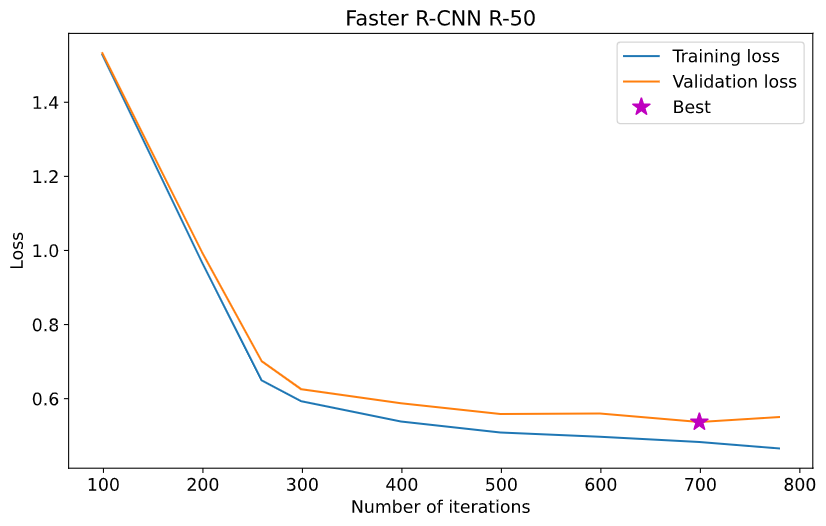
\includegraphics[width=\textwidth]{Sources/Figures/candies/Faster R-CNN R-50.png}
	\end{minipage}\hfill
	\begin{minipage}{0.5\textwidth}
		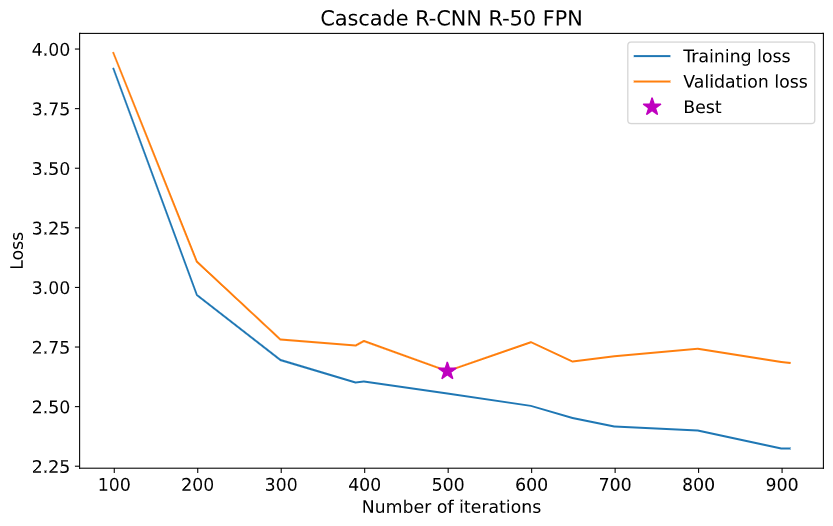
\includegraphics[width=\textwidth]{Sources/Figures/candies/Cascade R-CNN R-50 FPN.png}
	\end{minipage}\par
	\vskip\floatsep
	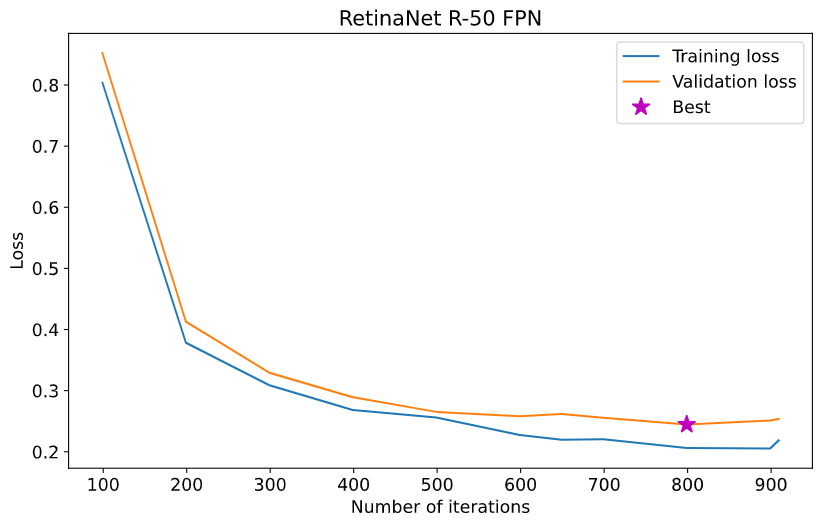
\includegraphics[width=0.5\textwidth]{Sources/Figures/candies/RetinaNet R-50 FPN.png}
	\caption{Loss curves of trained models on candies dataset.}
	\label{fig:candies_loss}
\end{figure}

\subsection{Metal parts dataset}
\begin{figure}[H]
	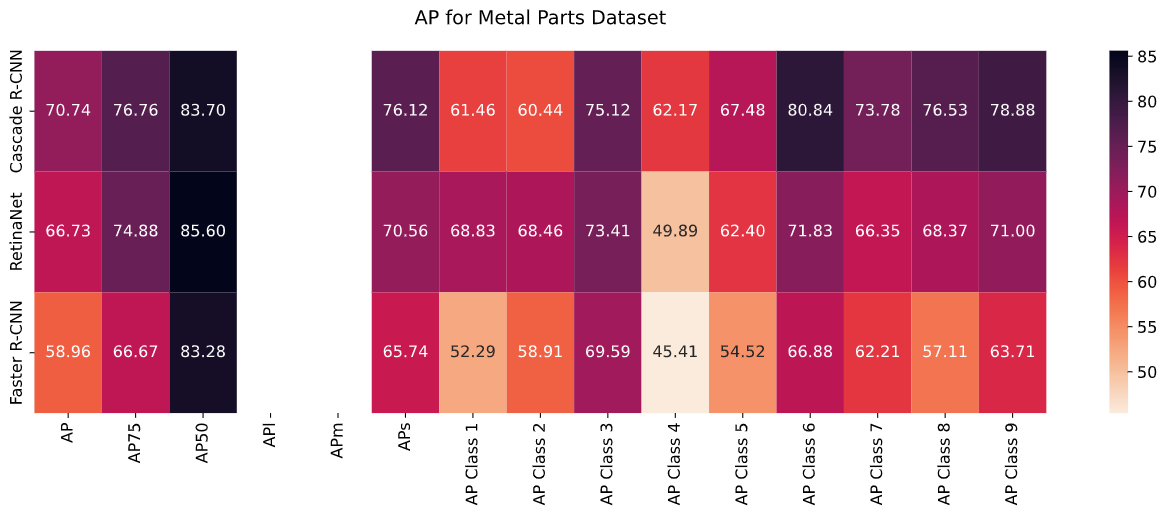
\includegraphics[width=\linewidth]{Sources/Figures/metal/metal_ap.png}
	\caption{AP table for metal parts dataset.}
\end{figure}

\begin{figure}[H]
	\centering
	\begin{minipage}{0.5\textwidth}
		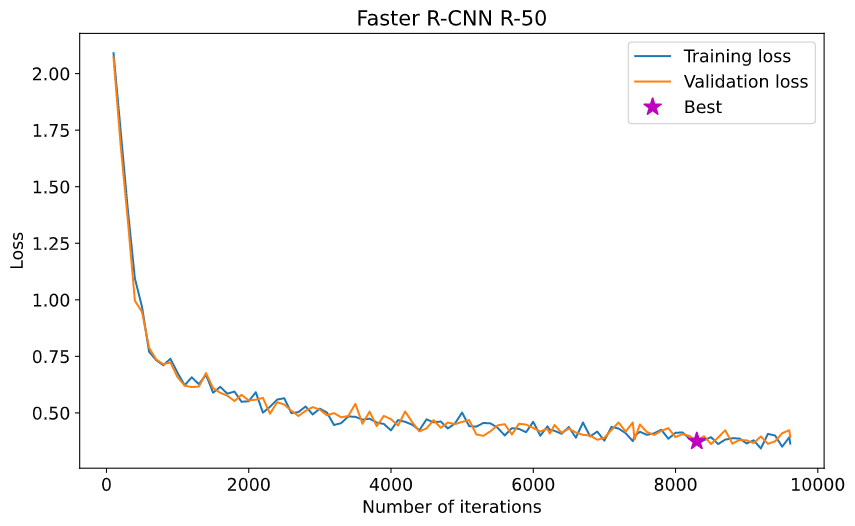
\includegraphics[width=\textwidth]{Sources/Figures/metal/metal_frcnn_loss.png}
	\end{minipage}\hfill
	\begin{minipage}{0.5\textwidth}
		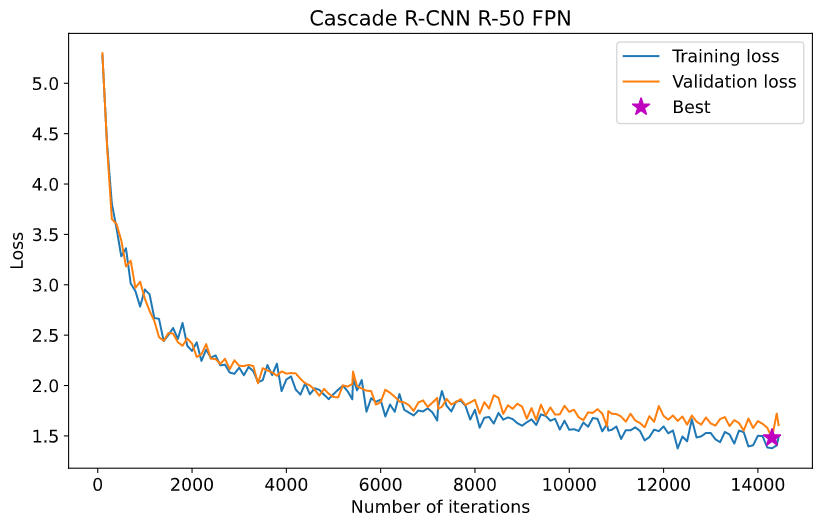
\includegraphics[width=\textwidth]{Sources/Figures/metal/metal_cascade_loss.png}
	\end{minipage}\par
	\vskip\floatsep
	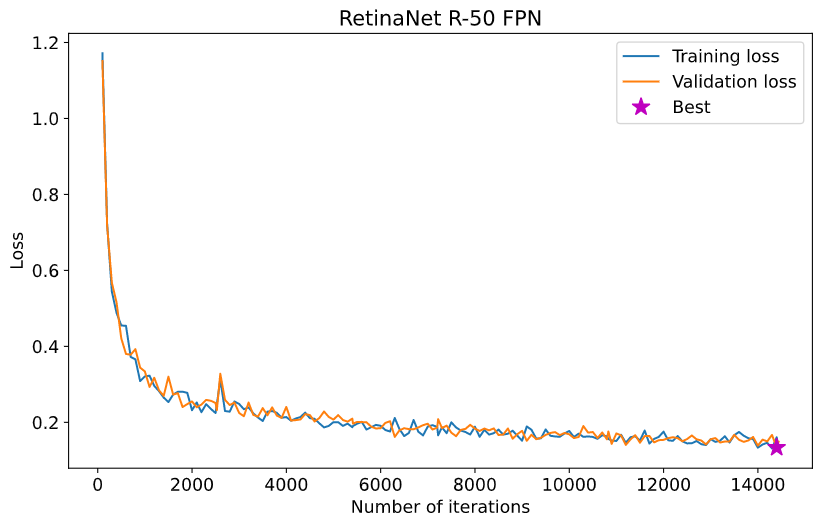
\includegraphics[width=0.5\textwidth]{Sources/Figures/metal/metal_retina_loss.png}
	\caption{Loss curves of trained models on metal parts dataset.}
	\label{fig:metal_loss}
\end{figure}

\subsection{Medical supplies dataset}

\begin{figure}[H]
	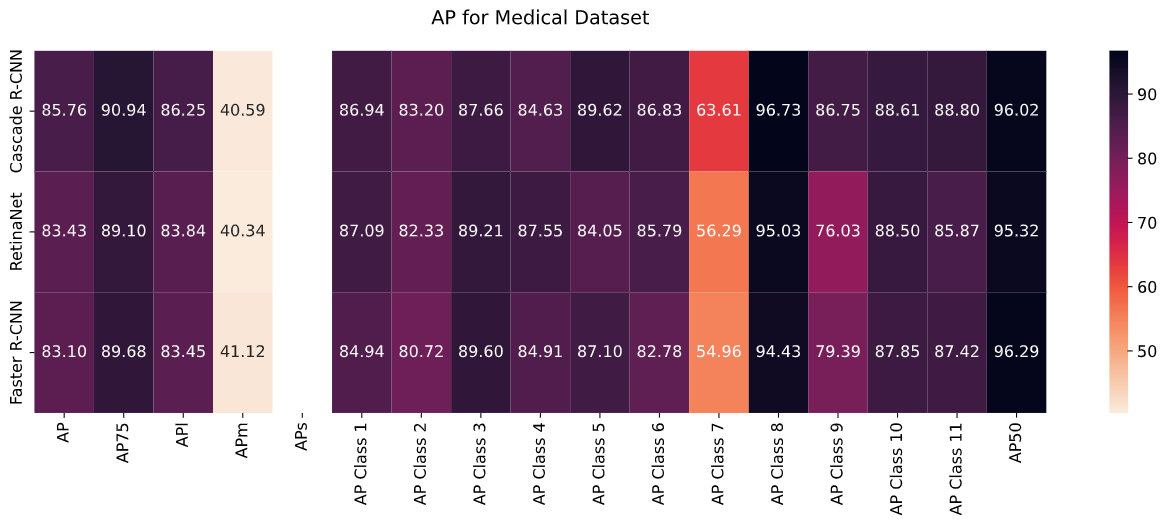
\includegraphics[width=\linewidth]{Sources/Figures/medical_ap_heatmap.png}
	\caption{AP table for medical dataset.}
\end{figure}

\begin{figure}[H]
	\centering
	\begin{minipage}{0.5\textwidth}
		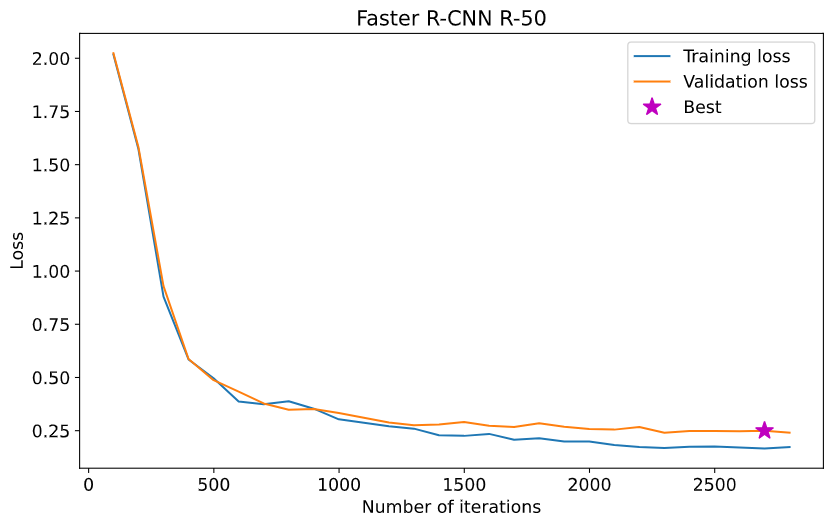
\includegraphics[width=\textwidth]{Sources/Figures/medical/frcnn_losses.png}
	\end{minipage}\hfill
	\begin{minipage}{0.5\textwidth}
		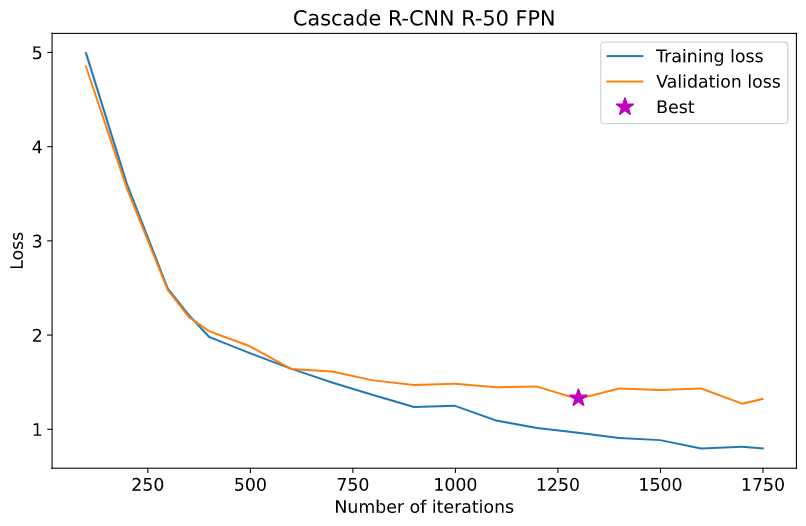
\includegraphics[width=\textwidth]{Sources/Figures/medical/cascade_losses.png}
	\end{minipage}\par
	\vskip\floatsep
	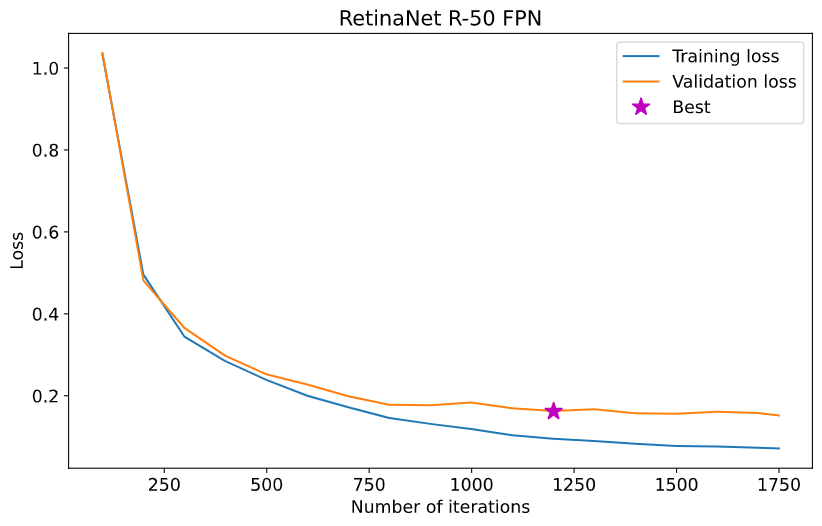
\includegraphics[width=0.5\textwidth]{Sources/Figures/medical/retina_losses.png}
	\caption{Loss curves of trained models on medical dataset.}
	\label{fig:medical_loss}
\end{figure}


\chapter{Benchmark Tool}
\begin{itemize}
    \item Vysvětlit usecase
    \item Design
    \item Použité technologie
\end{itemize}
To facilitate future evaluations of the models on new datasets, we have
"wrapped" the raw code used for our evaluation into a \bld{graphical user
    interface (GUI) application}. We have decided to implement the GUI as a
bld{web application}. This approach naturally solves the cross-platform (in
terms of operating systems) compatibility. On top of that, developing native
desktop applications can be very tedious; therefore, we have made this decision.
We believe that "running" a web application is more natural today.

As we mentioned, the GUI (\bld{frontend}) is implemented as a web application
with a JavaScript framework. The application's logic (\bld{backend}) is
implemented separately in Python and is accessed by HTTP requests. In the
following sections, we describe the application's design and implementation
details.

\section{Design}
The application's primary purpose is to train and evaluate selected models with
user-specified parameters on an arbitrary object detection dataset. We describe
the typical scenario of the user interaction with the application below:
\renewcommand{\theenumi}{\arabic{enumi}}
\begin{enumerate}
    \item The user uploads a new dataset or selects an old one. He can
          optionally define a split ratio by which the dataset will be split
          into training, test, and validation set.
    \item The user selects models to evaluate.
    \item The user sets models' parameters.
    \item The user initiates the training.
    \item The user then observes the results and eventually downloads the
          evaluation data.
\end{enumerate}
As we can see, the process can be split into a sequence of steps. Therefore, in
terms of the GUI design, we took inspiration from the layout of "setup wizards" (see Figure \ref{fig:wizard}).
At each step, only the relevant information is visible. The user can only go to
the previous or next step (if the user provides all the necessary information).

\begin{figure}[h]
    \centering
    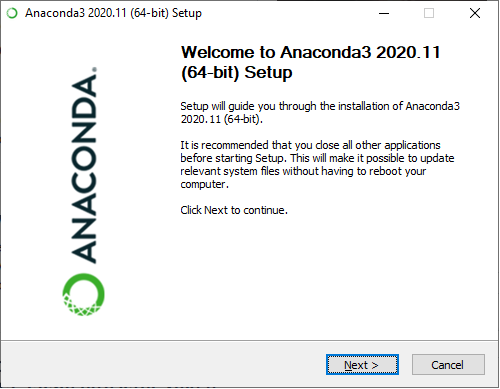
\includegraphics[width=0.65\linewidth]{Sources/Figures/anaconda.png}
    \caption{An example of a setup wizard.}
    \label{fig:wizard}
\end{figure}

The frontend communicates with the backend through the HTTP \bld{application
    programming interface (API)} composed of \bld{uniform resource identifier
    (URI)}
endpoints. The API will consist mainly GET and POST requests. For example, if we
would like to retrieve a list of datasets, we would send a GET request to a URI
of the form similar to \texttt{<api\_address>/datasets}. The POST requests will
be mainly used for setting up the training details and initiating the training
process. See Figure \ref{fig:tool_design} for an illustration of the communication.

\begin{figure}[h]
    \centering
    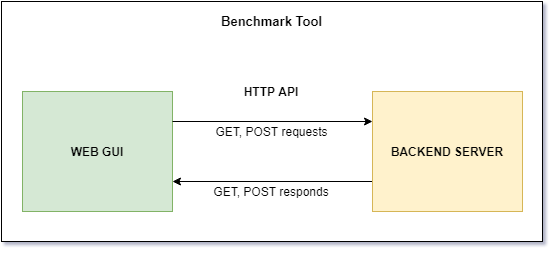
\includegraphics[width=0.85\linewidth]{Sources/Figures/tool_design.png}
    \caption{A diagram of bennchmark tool's design.}
    \label{fig:tool_design}
\end{figure}

\section{Implementation}
The frontend is developed in Vue.js. It is a JavaScript framework for building
interactive user interfaces. The interface is decomposed to many Vue components
that can communicate with each other and share the state. The structure of the
code is therefore more readable as it is written in a semantical hierarchy of
components. Each component is defined by its HTML template that can be extended
with JavaScript codes and Vue-specific special constructs (such as
\texttt{v-for} that can render elements of collections). For demonstration,
see Listing \ref{code:vue}. The \texttt{v-for} is added to the \texttt{<li>}
element and renders it for each item in \texttt{items} JavaScript array. The
\texttt{\{\{ item.message \}\}} is used for text interpolation that renders the
JavaScript value as a HTML text.

\begin{lstlisting}[language=HTML, caption=Vue.js template example]
<ul>
    <li v-for="item in items">
        {{ item.message }}
    </li>
</ul>
\end{lstlisting}
\label{code:vue}


% Fortunately, we could implement this layout with ease by using a Material Design
% Framework Vuetify that includes a "stepper" component that corresponds to the
% design as mentioned above.
\chapter{Conclusion}
Future work proposals
% This ensures that the subsequent sections are being included as root
% items in the bookmark structure of your PDF reader.
\bookmarksetup{startatroot}
\backmatter

%   \begingroup
%     \let\clearpage\relax
%     \glsaddall
%     % \printglossary[type=\acronymtype]
%     % \newpage
%     % \printglossary
%   \endgroup

\printindex
\begingroup
\sloppy
% \RaggedRight %% needs package ragged2e
\printbibliography
\endgroup

\end{document}
